\documentclass{article}
\usepackage{tabularx} % Pacote para tabelas ajustáveis
\usepackage[utf8]{inputenc}
\usepackage{sectsty}
\usepackage{titlesec}
\usepackage{geometry}
\usepackage{titling}
\usepackage{graphicx}
\usepackage{float}
\usepackage{multicol}
\usepackage{hyperref}
\hypersetup{
    colorlinks=true,
    linkcolor=black,
    filecolor=magenta,      
    urlcolor=blue,
    citecolor=black
    }

\geometry{top=1in, bottom=1in, left=1in, right=1in} 

\title{\fontsize{20}{20}\selectfont LabSaúde++\\} 
\author{Ana Luísa de Souza Paraguassu, 231003442\\
        Arthur da Silva Pereira Bispo,  232000490\\
        João Carlos Gonçalves de Oliveira Filho, 232009511\\
}
\date{}


\setlength{\droptitle}{-50pt} 

\begin{document}

\maketitle
\fontsize{12}{15}\selectfont % Define o tamanho da fonte do texto
\sectionfont{\fontsize{14}{18}\selectfont} % Tamanho da fonte da seção
\titlespacing{\section}{0pt}{30pt}{10pt} % Espaçamento antes e depois das seções


\vspace{mm}

\section{Descrição do Problema}
O projeto LabSaúde++ tem como objetivo desenvolver um sistema de gestão de logística interna para um laboratório de exames e vacinas. O sistema contará com uma interface gráfica, que visa facilitar a interação dos usuários administradores com a base de dados da empresa.

% \section{Interface}

% \begin{itemize}
%     \item O programa é inicializado com uma tela de login, que requer o CPF e a senha do usuário, dando acesso a tela de Gerenciamento, a tela do Atendente e a tela do Enfermeiro;
%     \item A tela de Gerenciamento permite ao administrador cadastrar, pesquisar e excluir(demitir) um funcionário, gerenciar o estoque de vacinas e os exames oferecidos pela clínica;
%     \item Na tela do Atendente, o funcionário é capaz de cadastrar, pesquisar e editar os dados dos pacientes, alterar os próprios dados, cadastrar agendamentos de exames e vacinas e realizar os pagamentos;
%     \item A tela do Enfermeiro permite ao funcionário alterar seus dados, acessar suas demandas, realizar os exames gerando laudos e aplicar vacinas gerando cartões de vacina.
% \end{itemize}

\section{Regras de Negócio}

\begin{itemize}
    \item O funcionamento do programa requer um login de administrador, responsável pelo cadastro de pelo menos 1 enfermeiro e 1 atendente;
    \item Os pacientes podem possuir um convênio associado ou não e, a depender do convênio, adquirir diferentes descontos no pagamento conforme a Tabela \ref{tab:convênios_coberturas_descontos};
    \item Pacientes idosos, ditos preferenciais, adquirem desconto pela idade.
\end{itemize}

        \begin{table}[H]
            \centering
            \caption{Convênios, coberturas e descontos oferecidos.}
            \label{tab:convênios_coberturas_descontos}
            \begin{tabularx}{\textwidth}{|X|X|X|c|}
            \hline
            Convênio & Exames Cobertos & Vacinas Cobertas & Desconto \\
            \hline
            Unimed & Dengue, Zika Vírus, Covid-19, Colesteral & Tríplice Viral, Hepatite B, Febre Amarela, HPV & 10\% \\
            \hline
            Amil & Zika Vírus, Covid-19, Sífilis, Ácido Úrico & Tríplice Viral, Dupla Adulto, Meningocócica ACWY & 15\% \\
            \hline
            Bradesco Saúde & Dengue, Sífilis, Rubéola, Toxoplasmose & Hepatite B, Dupla Adulto, Febre Amarela, HPV & 25\% \\
            \hline
            Porto Seguro & Dengue, Covid-19, Rubéola, Glicemia & Tríplice Viral, Hepatite B, Febre Amarela, Meningocócica ACWY & 30\% \\
            \hline
            \end{tabularx}
        \end{table}
    

% \section{Distribuição das Tarefas}
% \begin{itemize}
%     \item João: Responsável pelo desenvolvimento da tela de login, e das classes referentes às vacinas e disponibilização do cartão de vacina.
%     \item Ana: Responsável pelo desenvolvimento da classe exame e suas subclasses e telas referentes às mesmas.
%     \item Arthur: Responsável pelo desenvolvimento da classe Pessoa, suas subclasses e telas referentes às mesmas.
% \end{itemize}
\newpage

\section{Diagrama de Classes}
\vspace{10mm}
\begin{figure}[H]
    \centering
    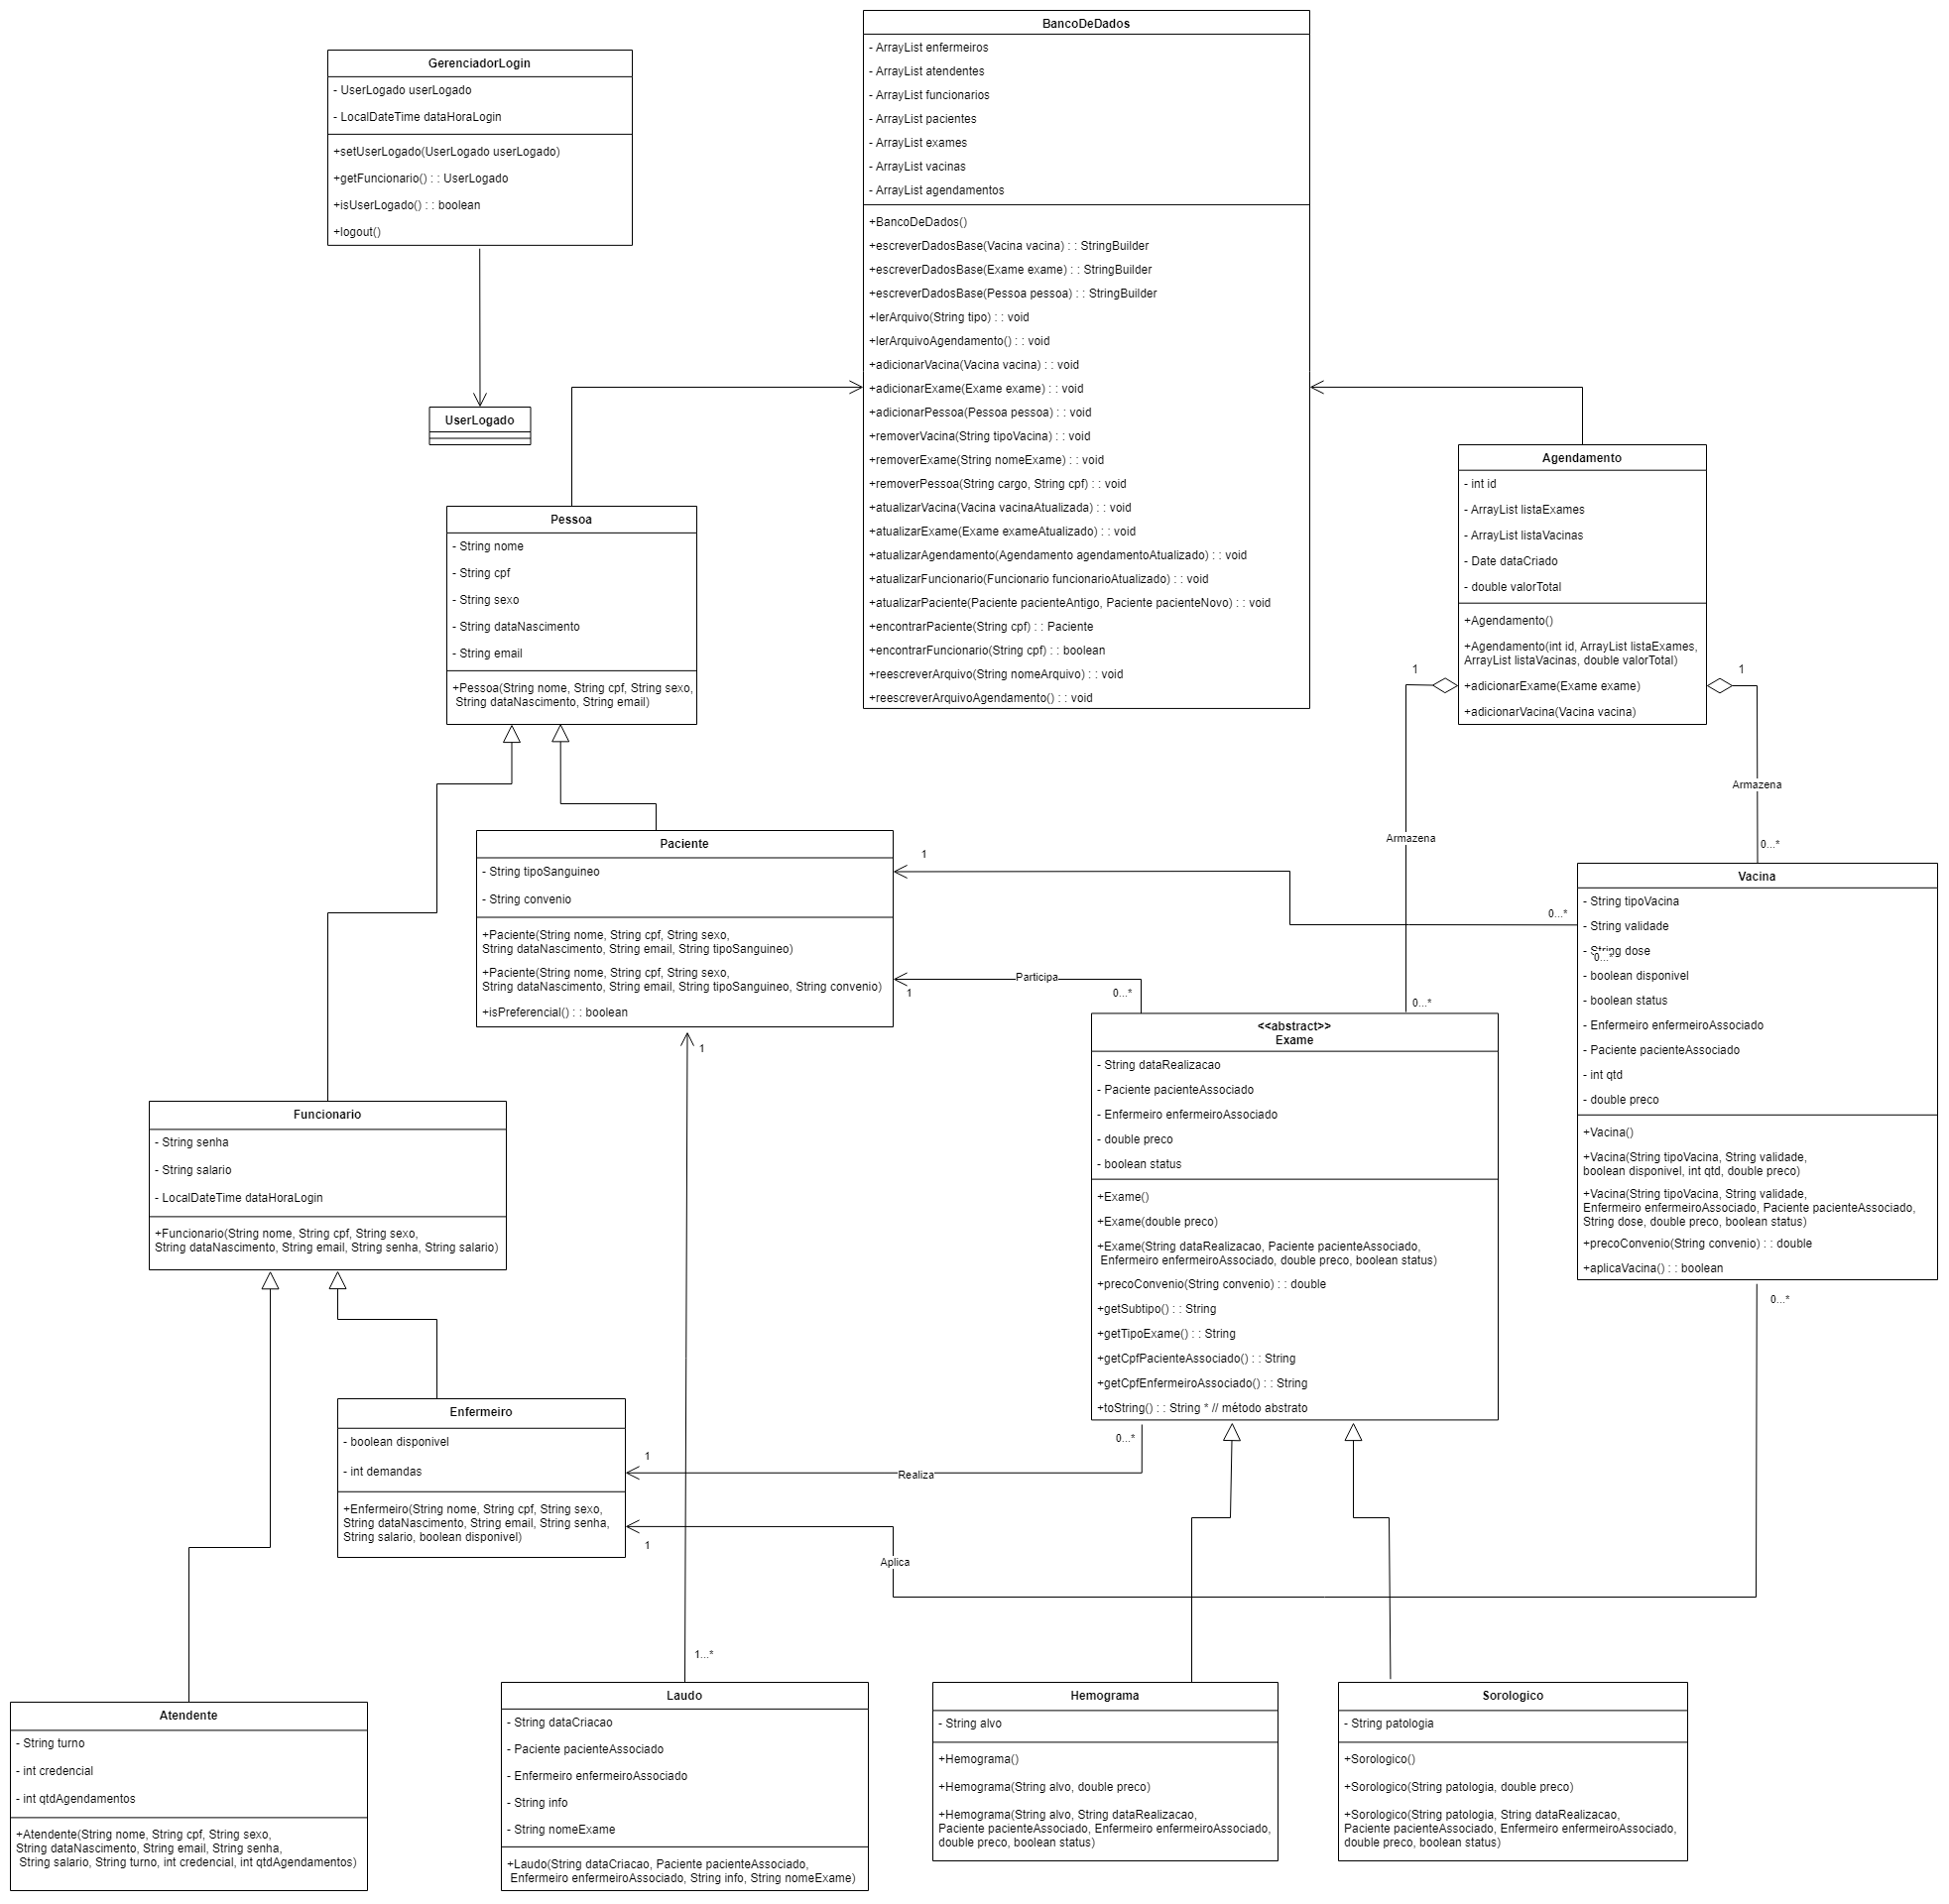
\includegraphics[width=17cm]{UML.drawio.png}
    \caption{Diagrama de classes final}
    \label{fig:diagrama}
\end{figure}

\newpage

\subsection{Descrição das Classes - atributos e métodos}
   \begin{itemize}

        \vspace{20mm}
        
        \item \textbf{Classe BancoDeDados}:
        Essa classe é responsável por toda a leitura e escrita de dados em arquivos CSV, sendo responsável por criar, ler, editar e excluir registros (CRUD). Ela organiza arquivos separados para cada tipo de entidade, como Funcionário, Atendente, Enfermeiro, Paciente, Exame, Vacina e Agendamento, garantindo que todas as informações do sistema fiquem bem armazenadas e acessíveis.
        
        \item \textbf{Classe Agendamento}: 
        Gerencia a lista de exames e vacinas de um paciente no sistema, com dados como data de criação e valor total. Permite adicionar novos exames e vacinas, e armazena suas informações.

        \item \textbf{Classe Pessoa}: 
        Superclasse para armazenar dados gerais de uma pessoa, como nome, CPF, sexo, data de nascimento e email.

        \item \textbf{Classe Funcionario}: 
        Superclasse para \texttt{Atendente} e \texttt{Enfermeiro}. Armazena informações como senha, salário e a data/hora do último login.
        
        \item \textbf{Classe Atendente}: 
        Representa um funcionário responsável pelo cadastro de pacientes e criação de agendamentos de exames e vacinas. Pode também editar dados de pacientes e visualizar resultados.
    
        \item \textbf{Classe Enfermeiro}: 
        Um funcionário que realiza exames e aplica vacinas. Contém um atributo de disponibilidade com base no número de demandas.

        \item \textbf{Classe Paciente}: 
        Representa um paciente cadastrado no sistema, com atributos como tipo sanguíneo e convênio, além de um método que verifica se o paciente é preferencial (idoso).
    
        \item \textbf{Classe Exame}: 
        Classe abstrata que representa exames médicos, contendo atributos como data de realização, paciente e enfermeiro associados, preço e status de conclusão.

        \item \textbf{Classe Hemograma}: 
        Classe especializada que herda de \texttt{Exame}, usada para representar exames do tipo hemograma.

        \newpage 
        
        \item \textbf{Classe Sorologico}: 
        Herda de \texttt{Exame} e representa exames sorológicos focados em patologias específicas.

        \item \textbf{Classe Vacina}: 
        Representa vacinas no sistema, com atributos como tipo, validade, dose, disponibilidade, preço e status de aplicação.

        \item \textbf{Classe Laudo}: 
        Representa um relatório de exame, com informações como data de criação, paciente, enfermeiro e o exame realizado.
    
        \item \textbf{Classe GerenciadorLogin}: 
        Implementa o padrão Singleton, que garante que apenas uma única instância da classe seja criada durante a execução do programa. Isso assegura que somente um login possa estar ativo no sistema por vez. A classe também armazena as informações do usuário logado e registra a data e hora em que o login foi realizado.

        \item \textbf{Interface UserLogado}:
        Interface que define as operações básicas para identificar o funcionário logado no sistema. Implementada pela classe Funcionario para fornecer informações do usuário autenticado e a data/hora do login.
    
    \end{itemize}


\section{Descrição da Telas}

\vspace{10mm}

\subsection{Parte Inicial}
    \begin{multicols}{2}
        \begin{figure}[H]
            \centering
            
\includegraphics[width=8cm]{Tela_Inicial.png}
            \caption{Tela inicial}
        \end{figure}
        
        A tela Inicial é apenas uma apresentação do programa a 
        ser explorado nas telas seguintes.
        
        \begin{figure}[H]
            \centering
            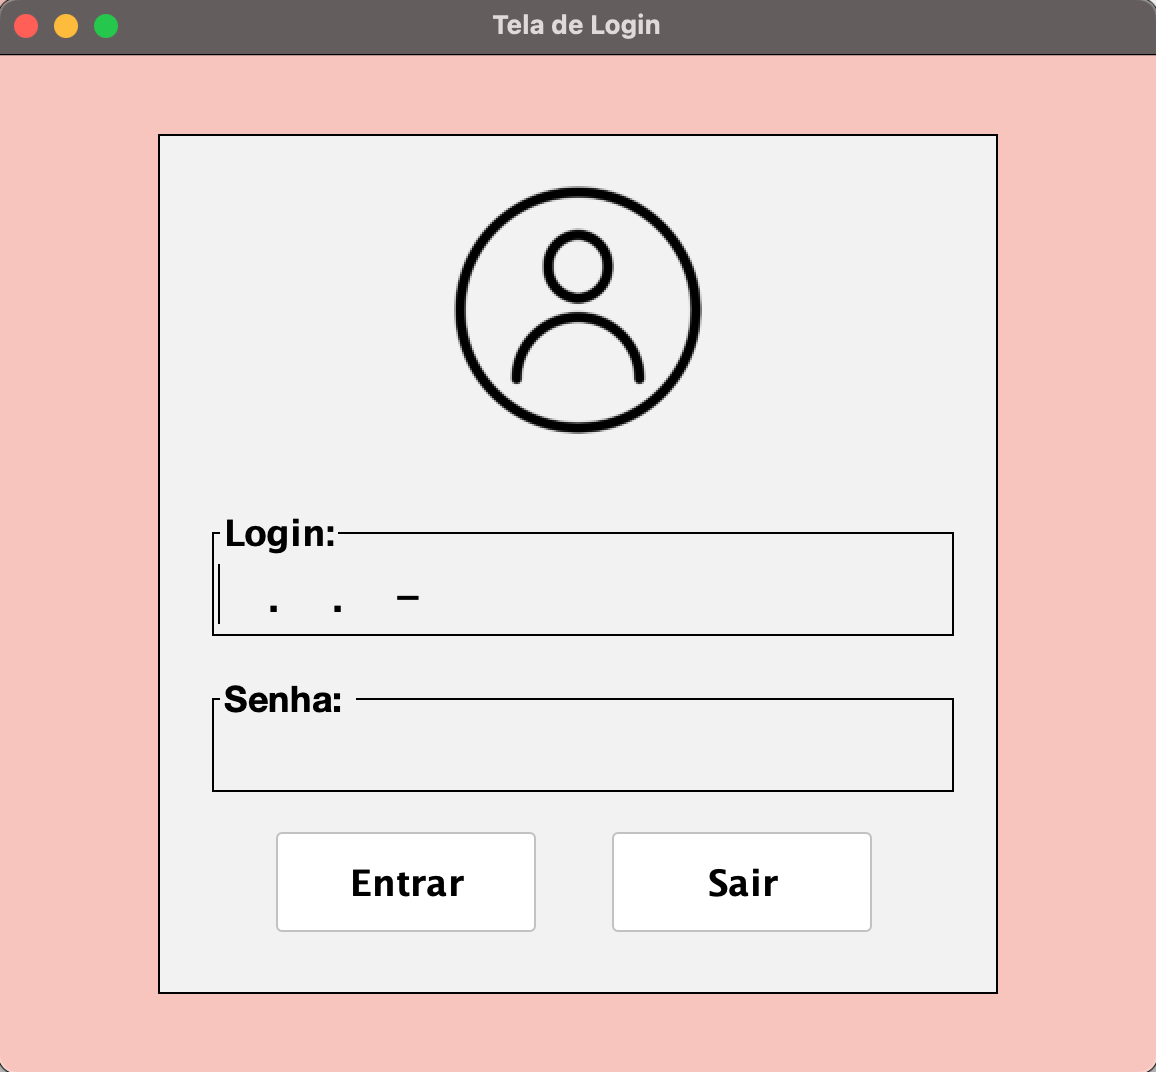
\includegraphics[width=6cm]{telaLogin.png}
            \caption{Tela de Login}
        \end{figure}
    
        A tela Login permite ao usuário acessar sua área de trabalho a partir de um login (CPF) e uma senha. A existência desses dados é verificada no Banco de Dados para liberar o acesso. 
    
    \end{multicols}

\subsection{Parte Administrador}
    \begin{figure}[H]
        \centering
        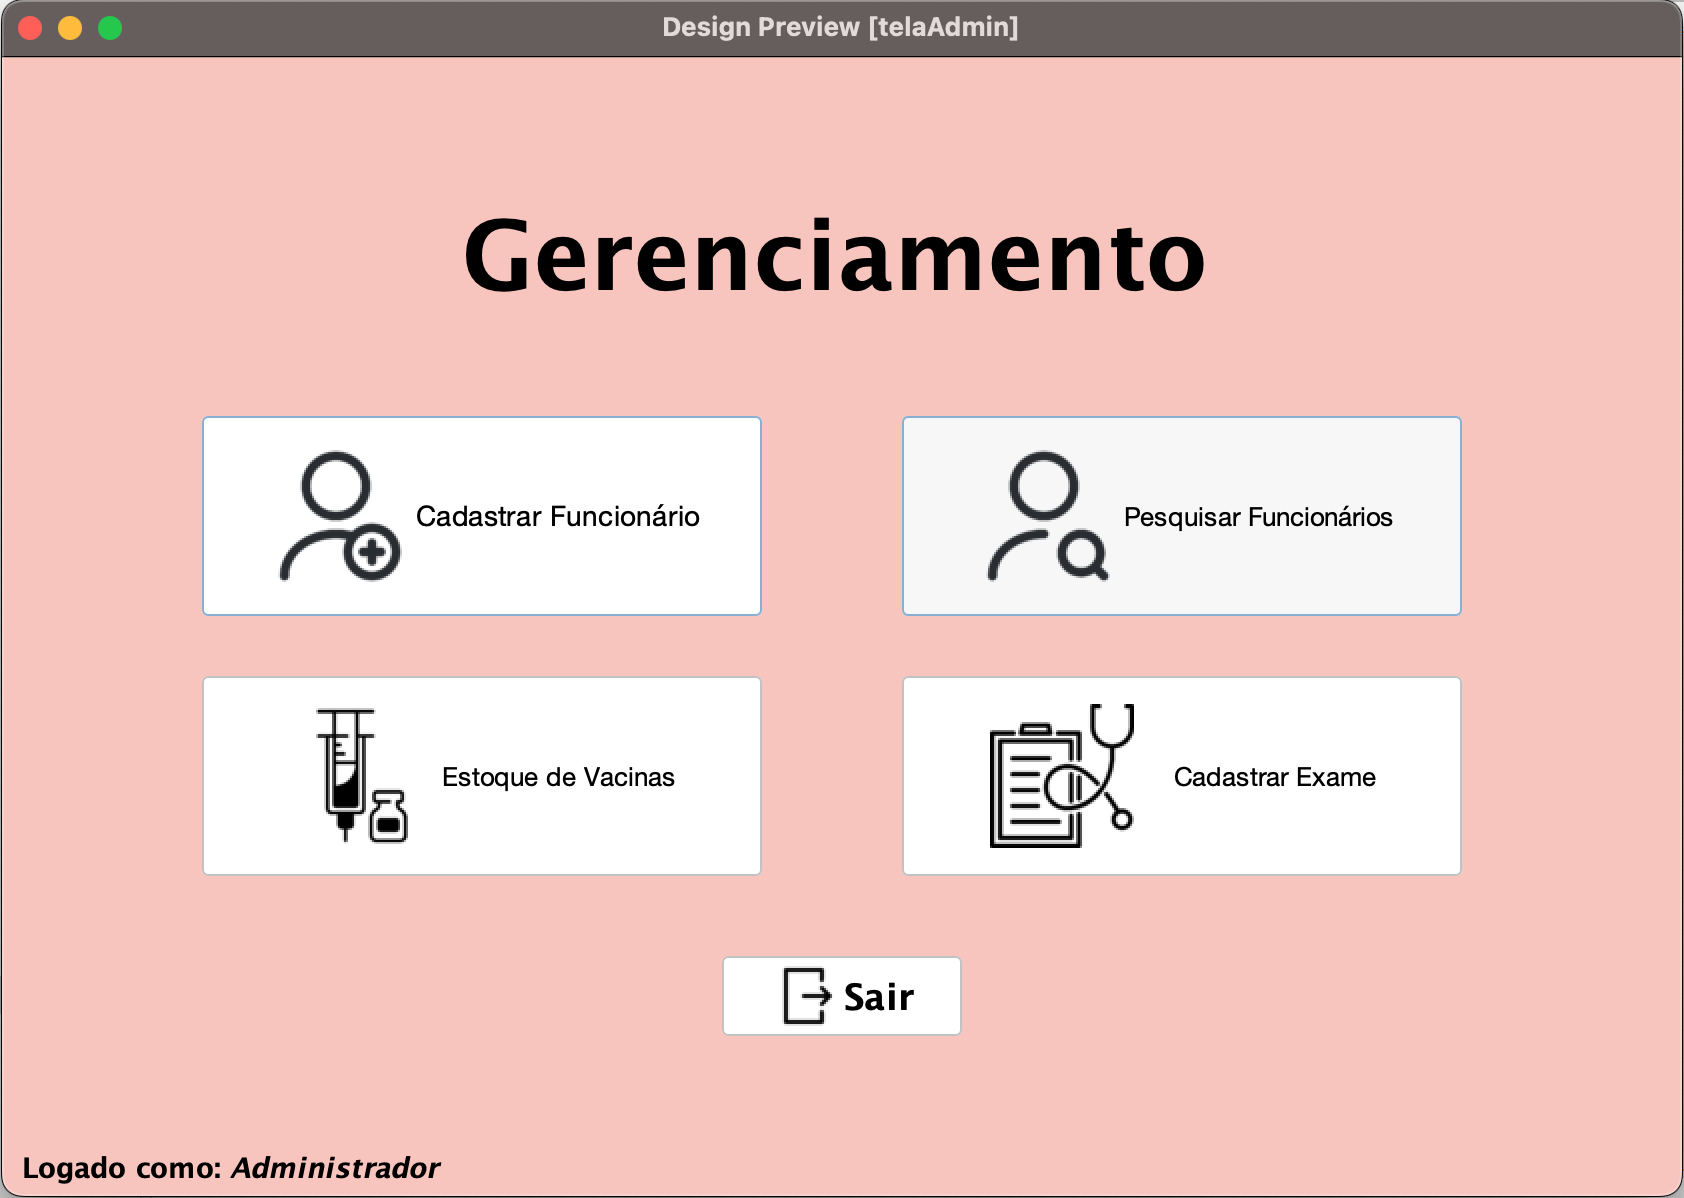
\includegraphics[width=10cm]{telaAdm.png}
        \caption{Tela Administrador}
    \end{figure}
    
    Essa tela é responsável pela conexão das principais funções do usuário Administrador, sendo: o cadastro e a pesquisa de funcionários, e o cadastro, edição, pesquisa e deleção de exames.
    
    \begin{multicols}{2}
    
        \begin{figure}[H]
            \centering
            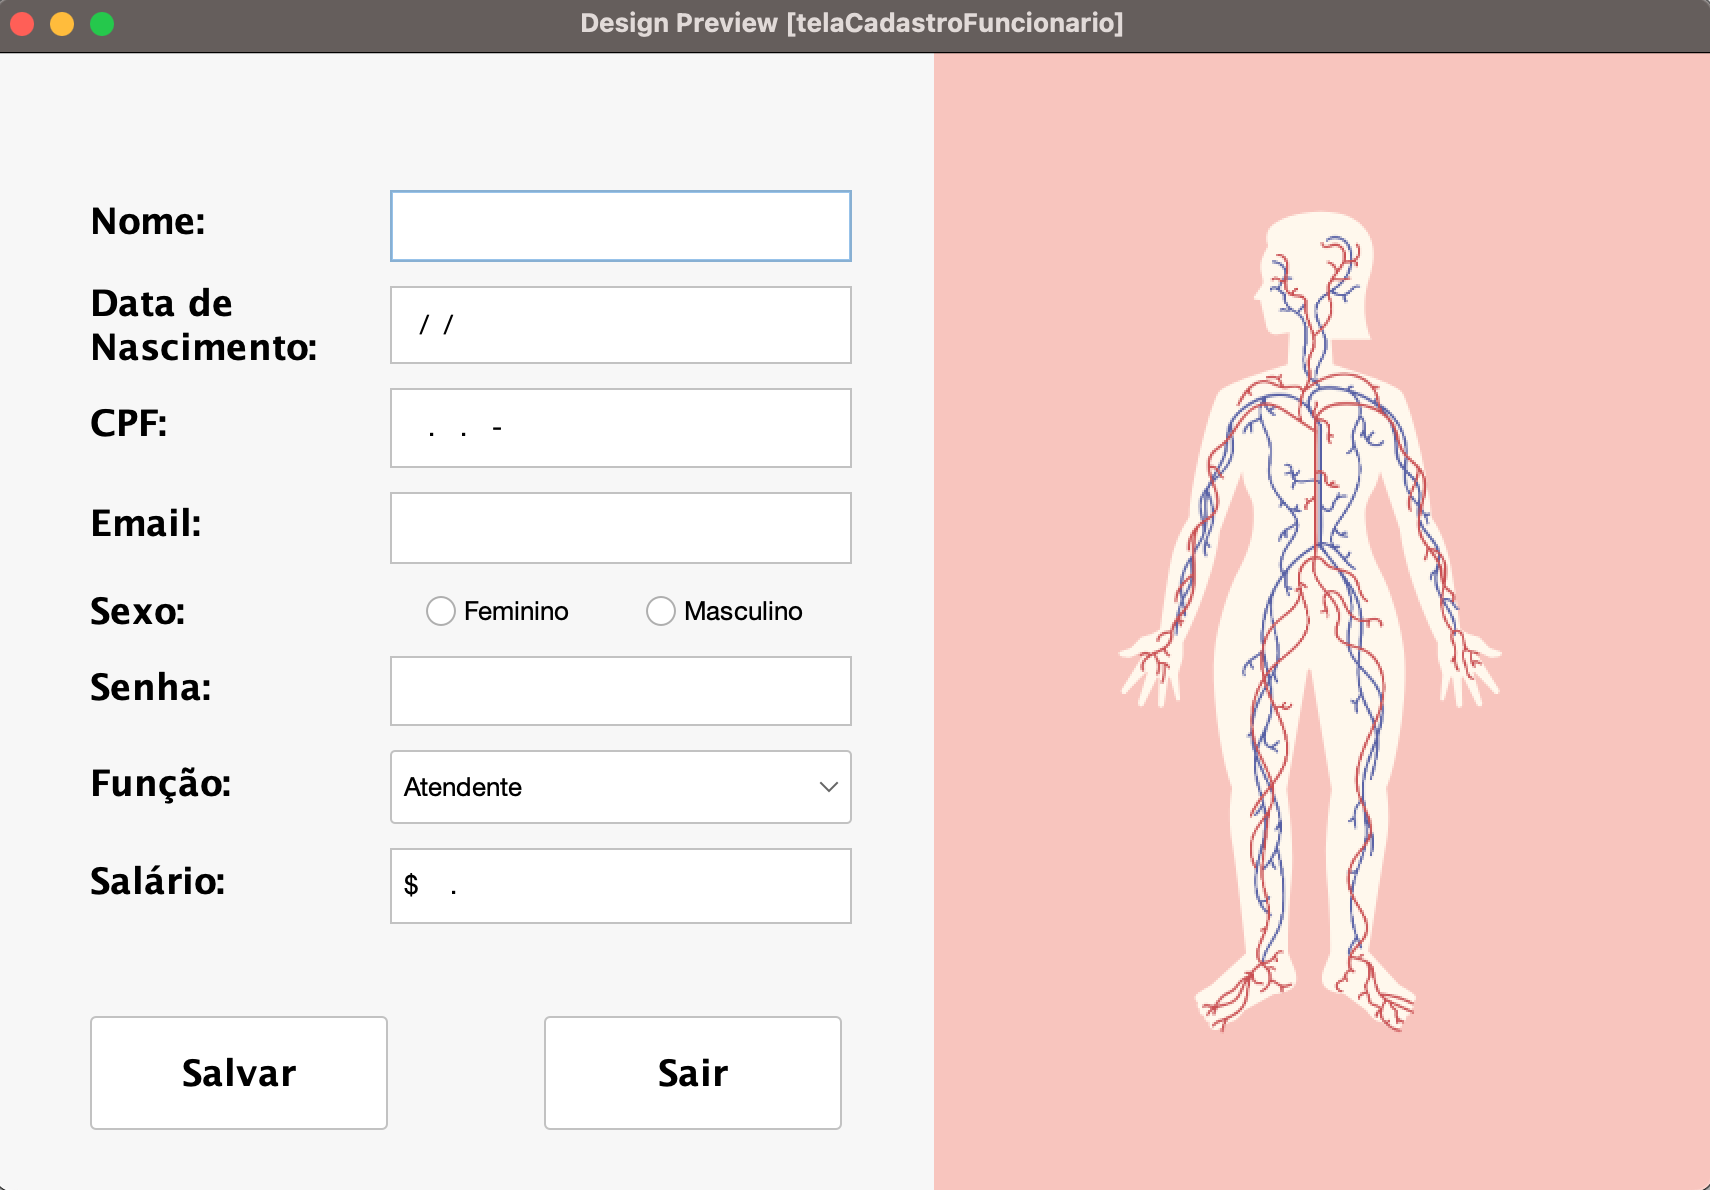
\includegraphics[width=8cm]{telaCadastroFuncionario.png}
            \caption{Tela Cadastro Funcionário}
        \end{figure}

        Esta tela registra os funcionários na base de dados do programa, possibilitando a especificação dos atributos e função (atendente ou enfermeiro).
        
        \begin{figure}[H]
            \centering
            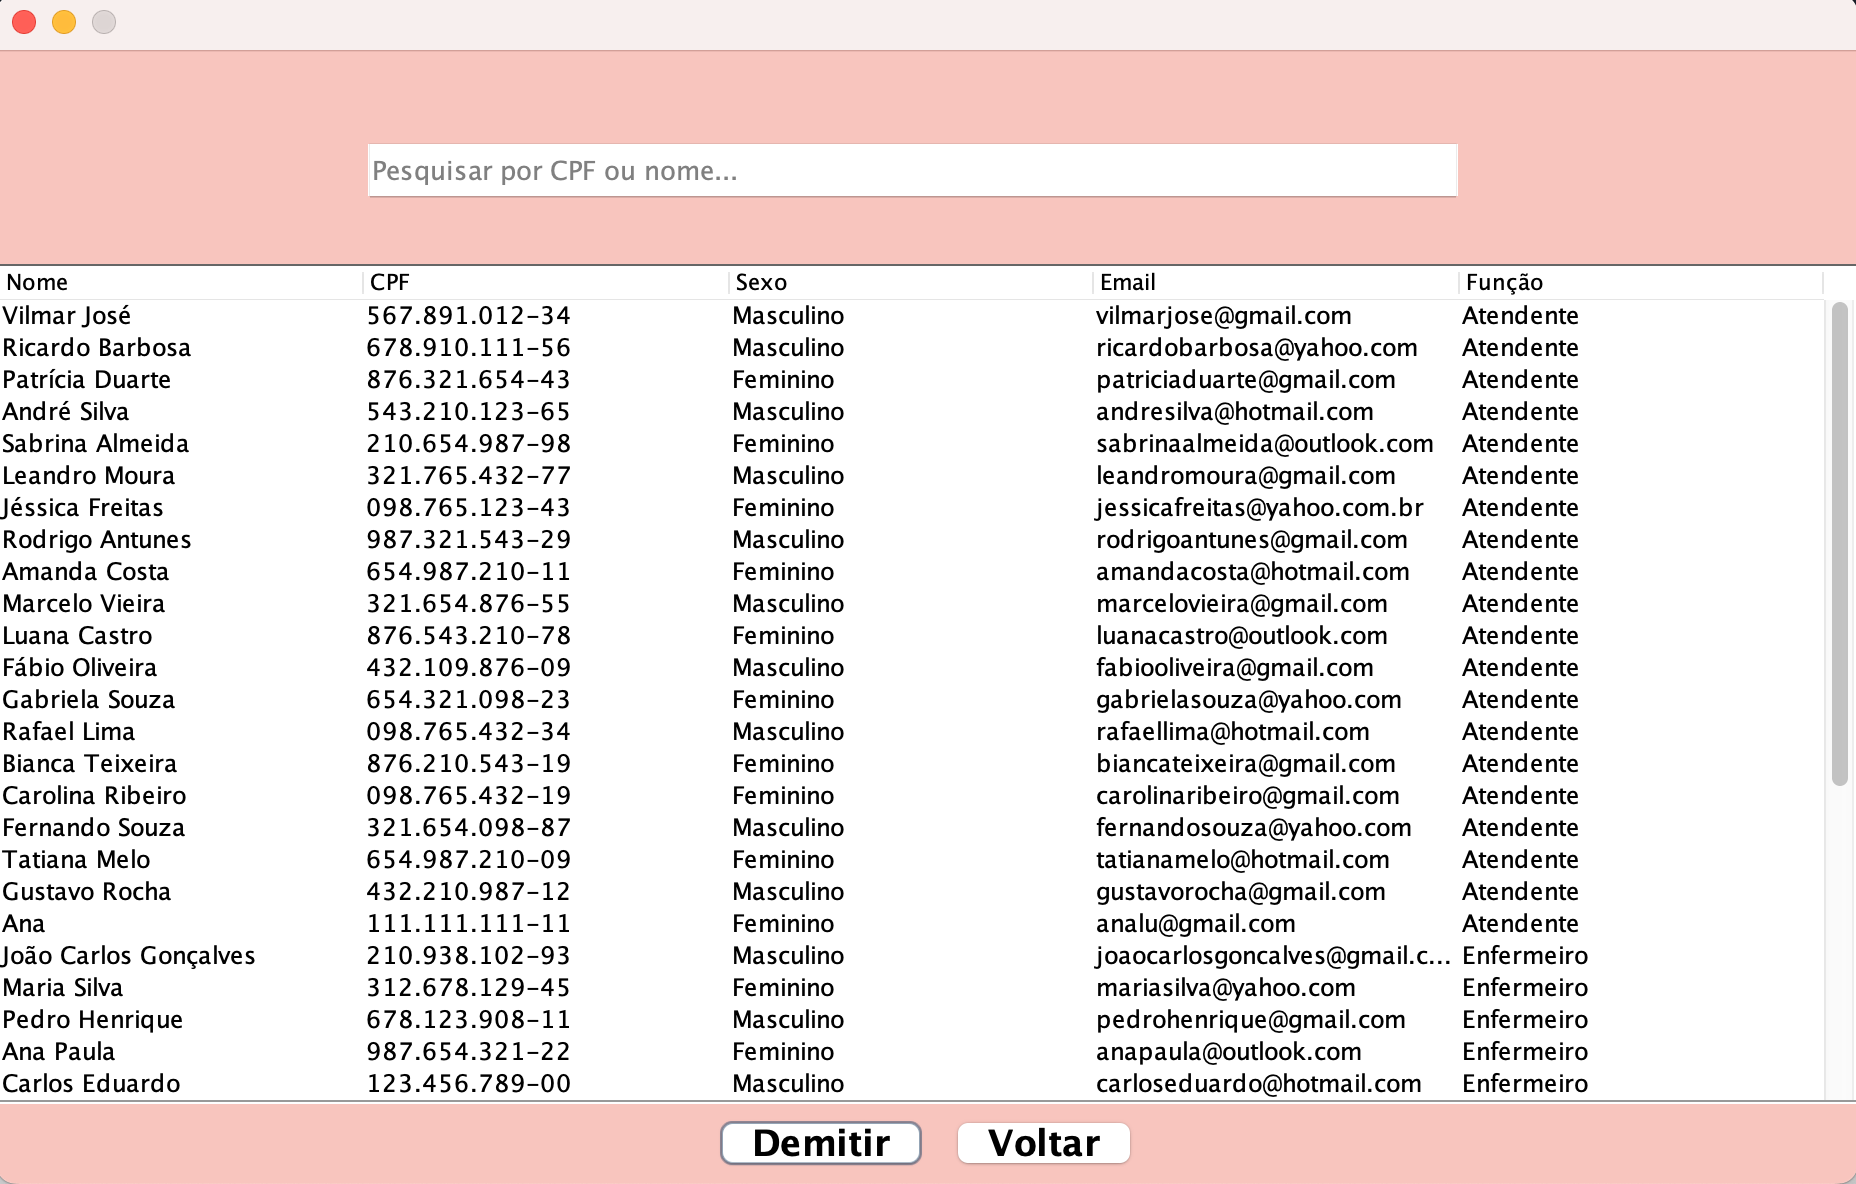
\includegraphics[width=8cm]{telaPesquisarFuncionario.png}
            \caption{Tela Pesquisar Funcionário}
        \end{figure}

       A tela Pesquisar Funcionário serve para a pesquisa de funcionários cadastrados no banco de dados. A pesquisa pode ser realizada pelo CPF ou pelo Nome. Além disso, esta tela também permite demitir/excluir um funcionário. 
        
        \begin{figure} [H]
            \centering
            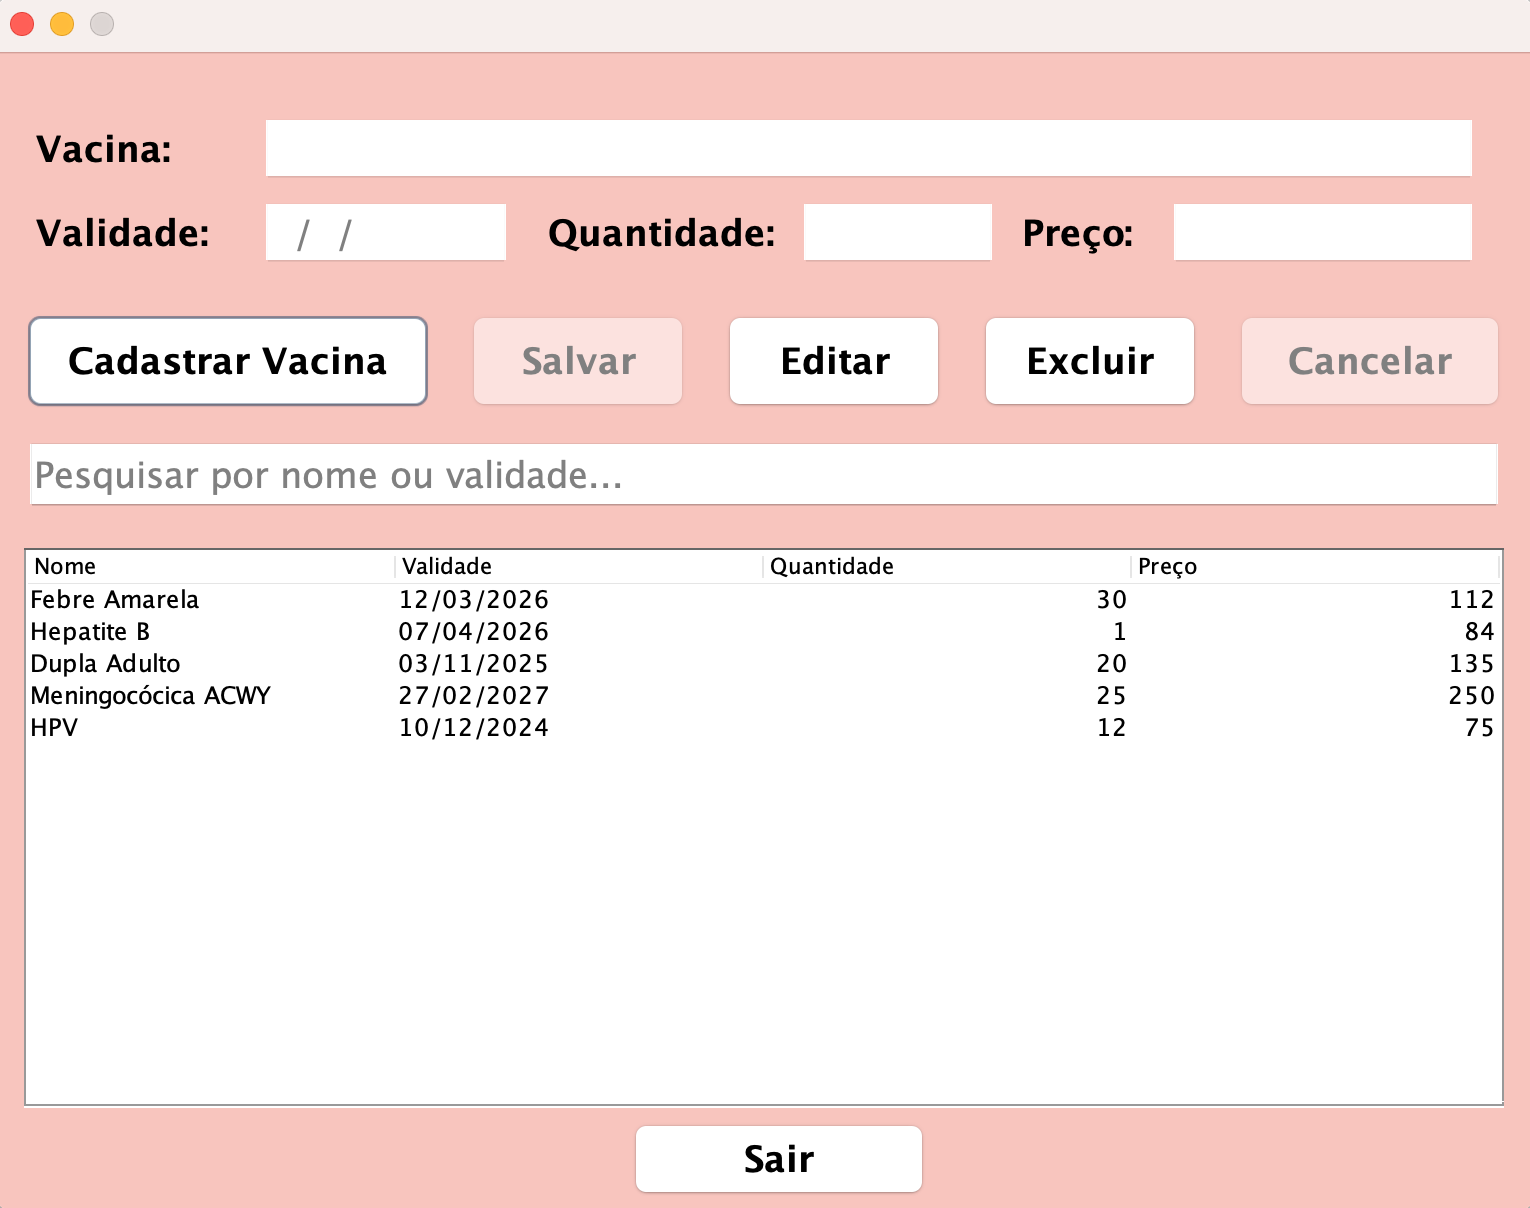
\includegraphics[width=8cm]{telaEstoqueVacina.png}
            \caption{Tela Estoque Vacina}
        \end{figure}

        A tela Estoque Vacina é destinada ao gerenciamento de vacinas no banco de dados. Ela permite a criação, edição, pesquisa e exclusão de vacinas já existentes.
        
        \begin{figure}[H]
            \centering
            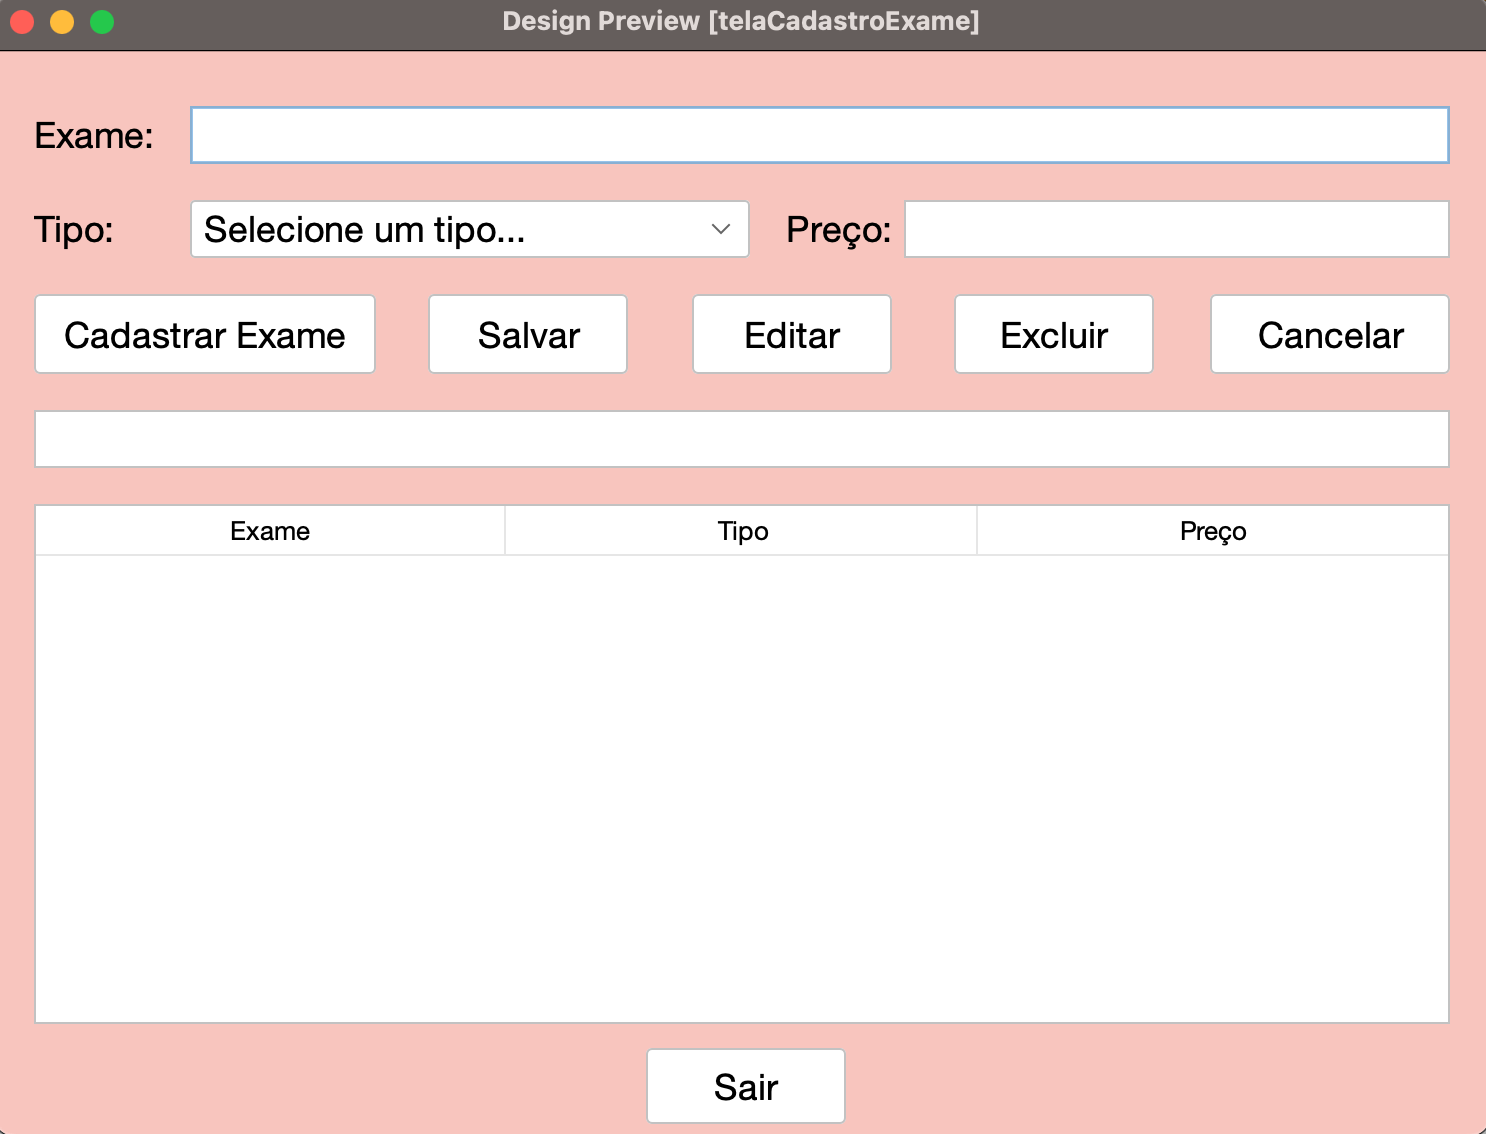
\includegraphics[width=8cm]{telaCadastroExame.png}
            \caption{Tela Cadastro Exame}
        \end{figure}

        Essa tela é destinada ao cadastro de exames no banco de dados. Nela, é possível criar, excluir, editar e pesquisar exames já existentes.
        
    \end{multicols}


\subsection{Parte Atendente}

    \vspace{10mm}

    \begin{figure}[H]
        \centering
        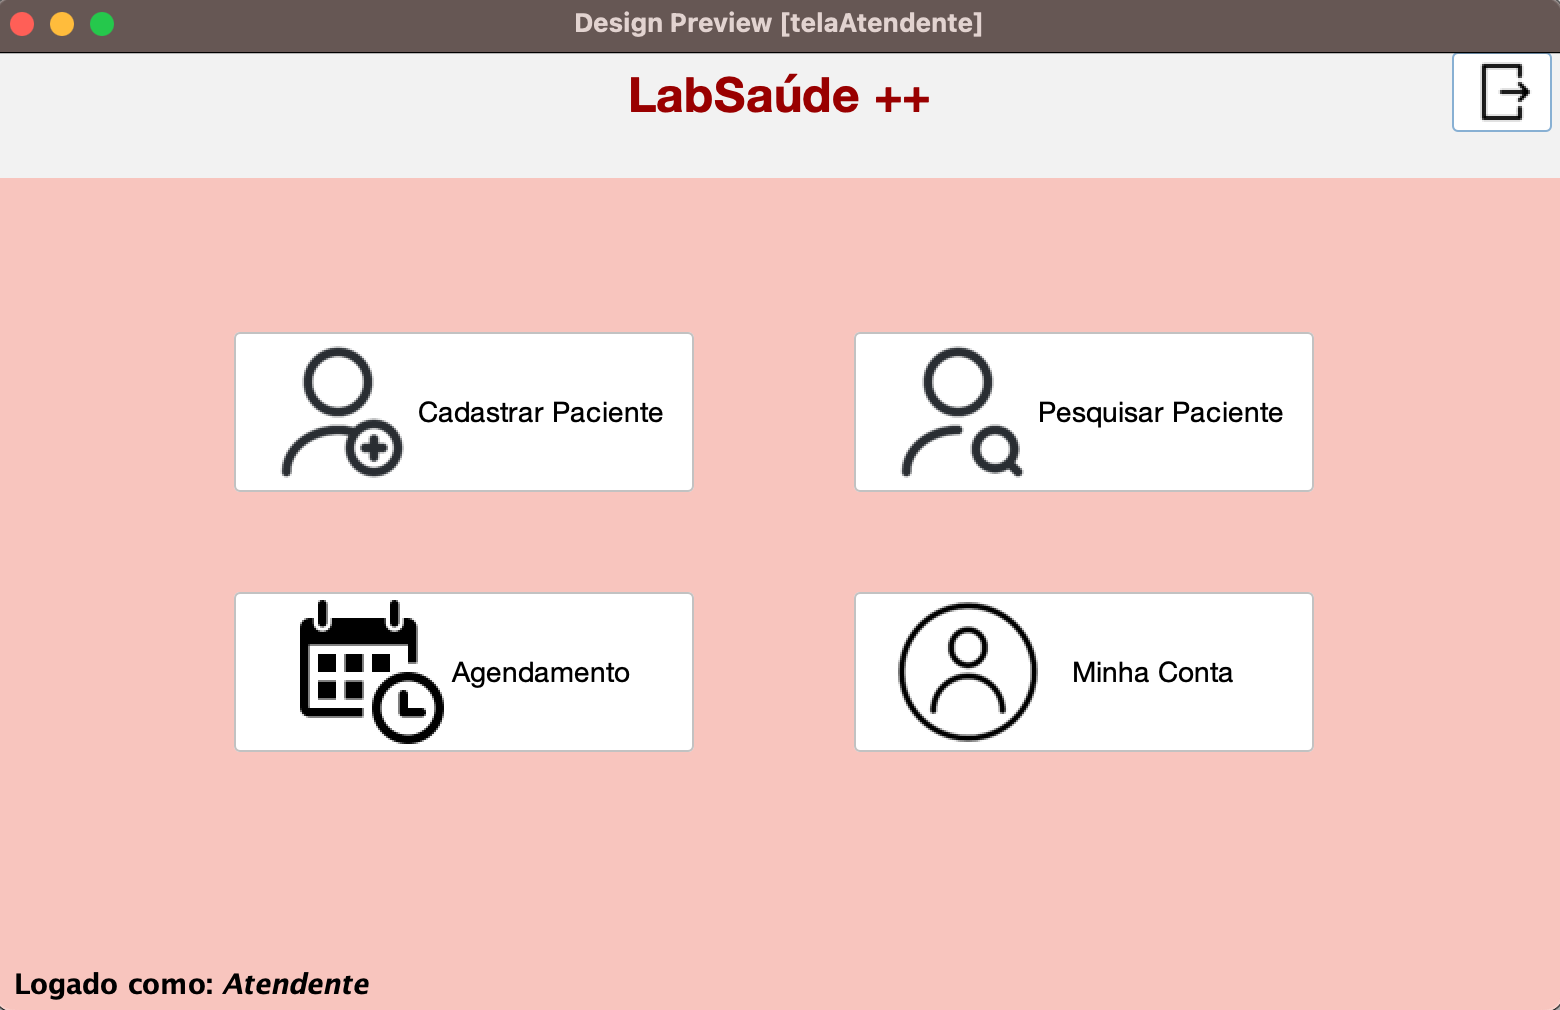
\includegraphics[width=10cm]{telaAtendente.png}
        \caption{Tela Atendente}
    \end{figure}
    
    Essa tela é responsável pela conexão das principais funções do usuário Atendente, que são: cadastrar, pesquisar e editar pacientes, agendar exames e vacinas, finalizar pagamentos, e alterar os dados da própria conta - Tela Conta Funcionário (\ref{Figure 19}).
    
    \begin{multicols}{2}
    
        \begin{figure}[H]
            \centering
            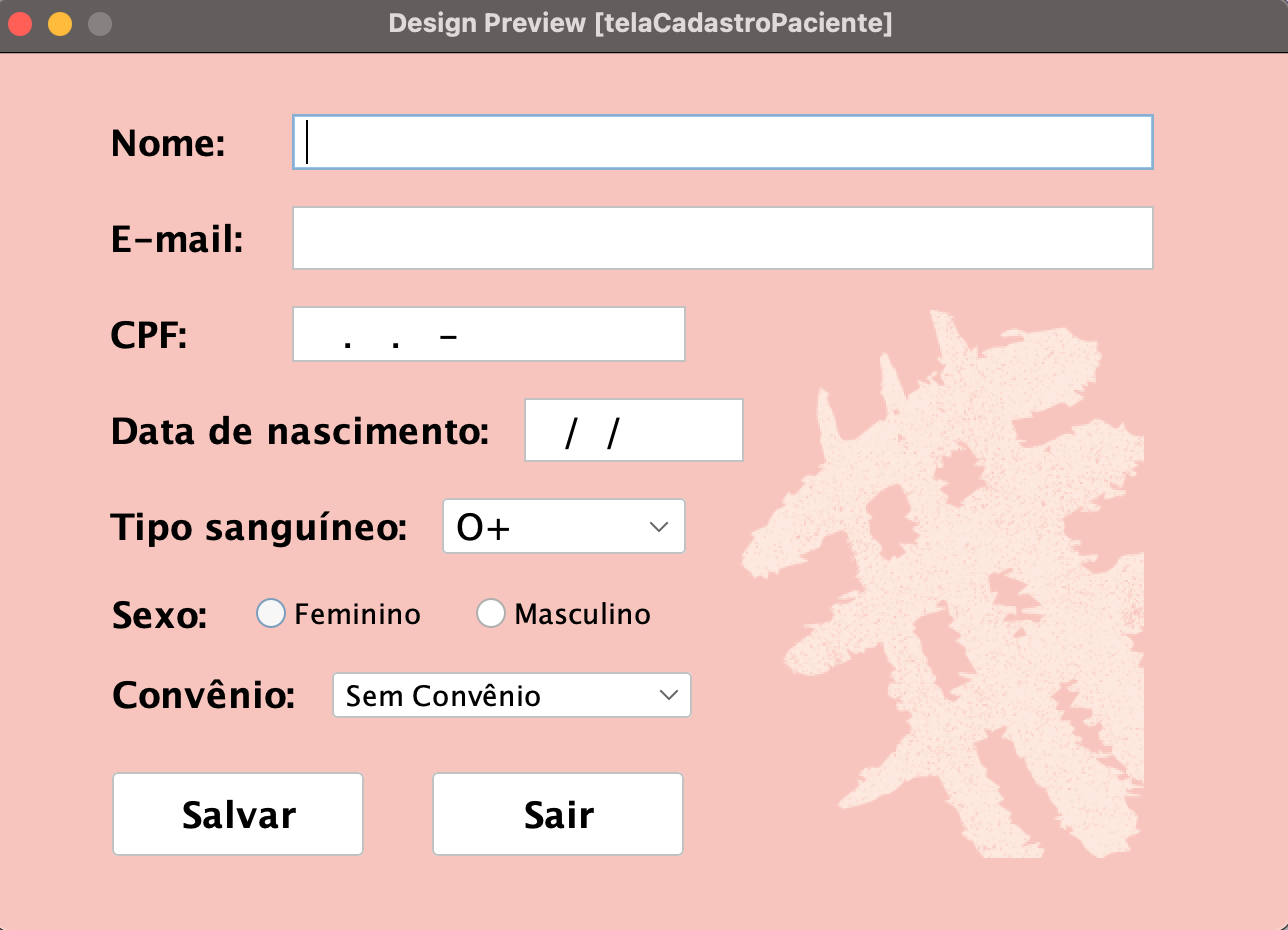
\includegraphics[width=8cm]{telaCadastroPaciente.png}
            \caption{Tela Cadastro Paciente}
            \label{Figure 9}
        \end{figure}
        
        A tela Cadastro Paciente permite inserir e armazenar dados de pacientes no sistema, incluindo nome, e-mail, CPF, data de nascimento, tipo sanguíneo, sexo e convênio, auxiliando no gerenciamento eficiente dessas informações.
        
        \begin{figure}[H]
            \centering
            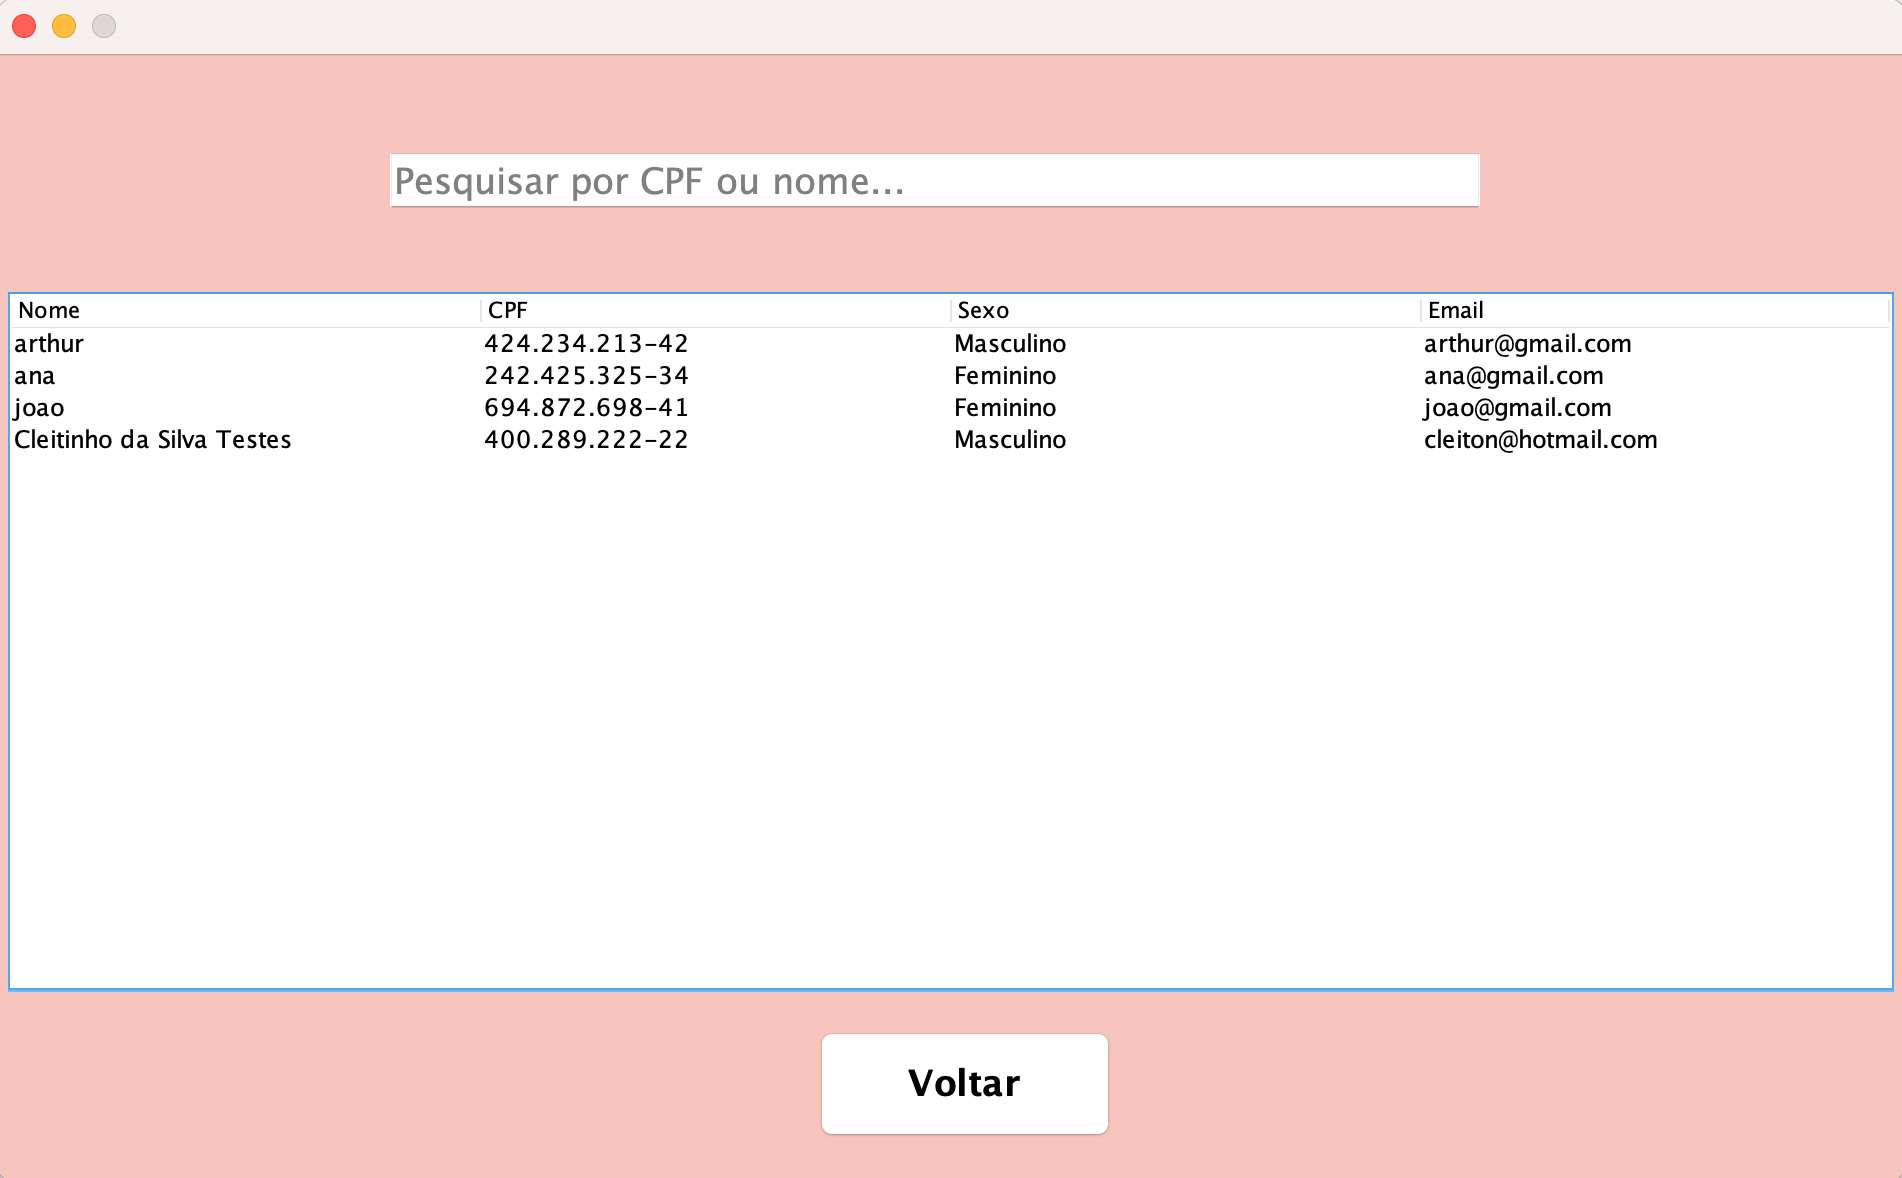
\includegraphics[width=8cm]{telaPesquisarPaciente.png}
            \caption{Tela Pesquisar Paciente}
        \end{figure}

        A tela Pesquisar Paciente possibilita a pesquisa de pacientes por CPF ou por nome e, ao selecionar um paciente, é possível editar seus dados em um pop-up da tela Cadastro Paciente (\ref{Figure 9}).
        
        \begin{figure}[H]
            \centering
            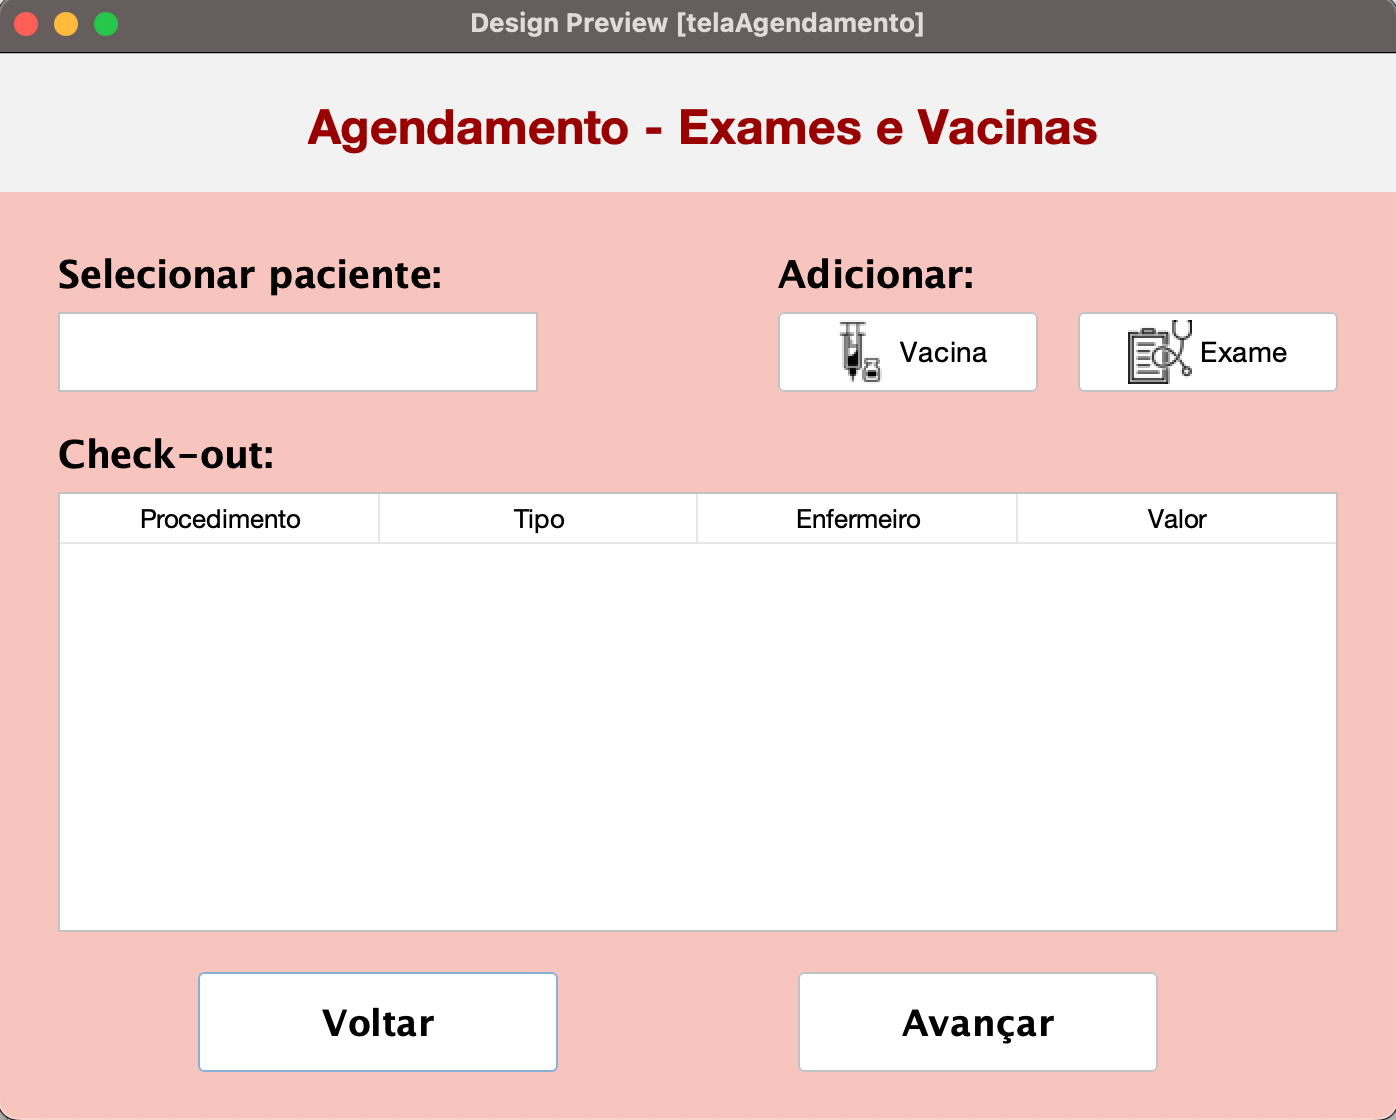
\includegraphics[width=8cm]{telaAgendamento.png}
            \caption{Tela Agendamento}
        \end{figure}

        Essa tela permite ao atendente gerir e exibir os agendamentos dos pacientes - adicionando exames e vacinas ao check-out, prosseguindo para o pagamento (\ref{Figure 14}).
        
        \begin{figure}[H]
            \centering
            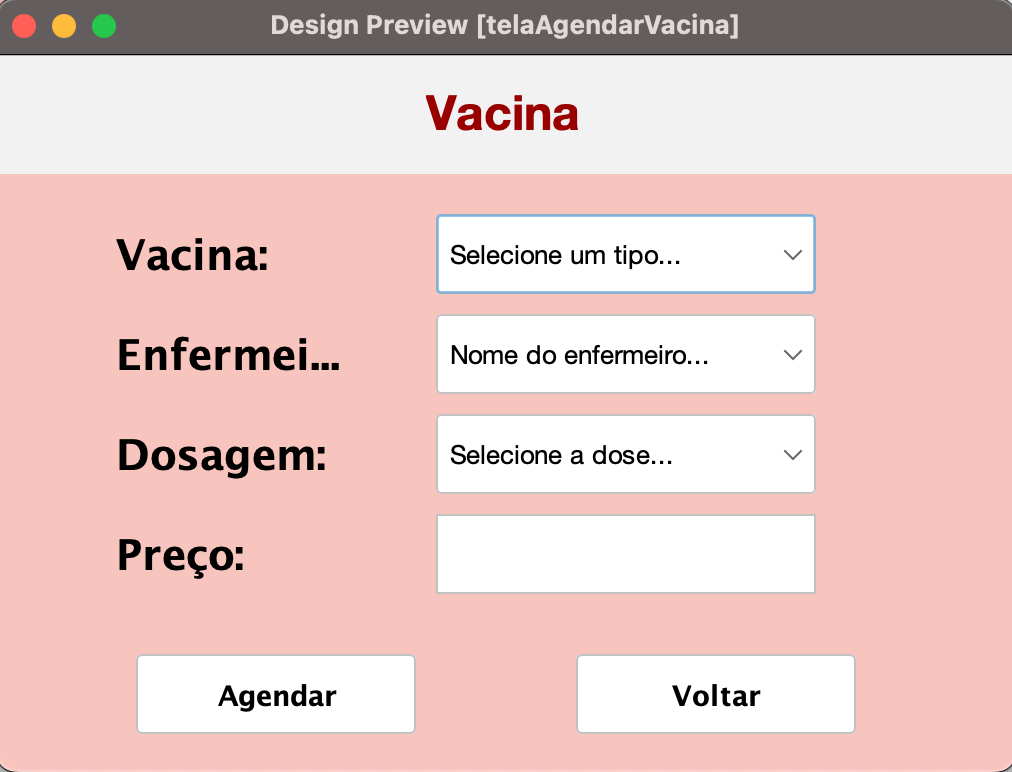
\includegraphics[width=8cm]{telaAgendarVacina.png}
            \caption{Tela Agendar Vacina}
        \end{figure}

        A tela Agendar Vacina facilita o preenchimento dos dados necessários para o agendamento de vacinas, permitindo: definir a vacina específica, o enfermeiro responsável e a dosagem, e visualizar o preço.
        
        \begin{figure}[H]
            \centering
            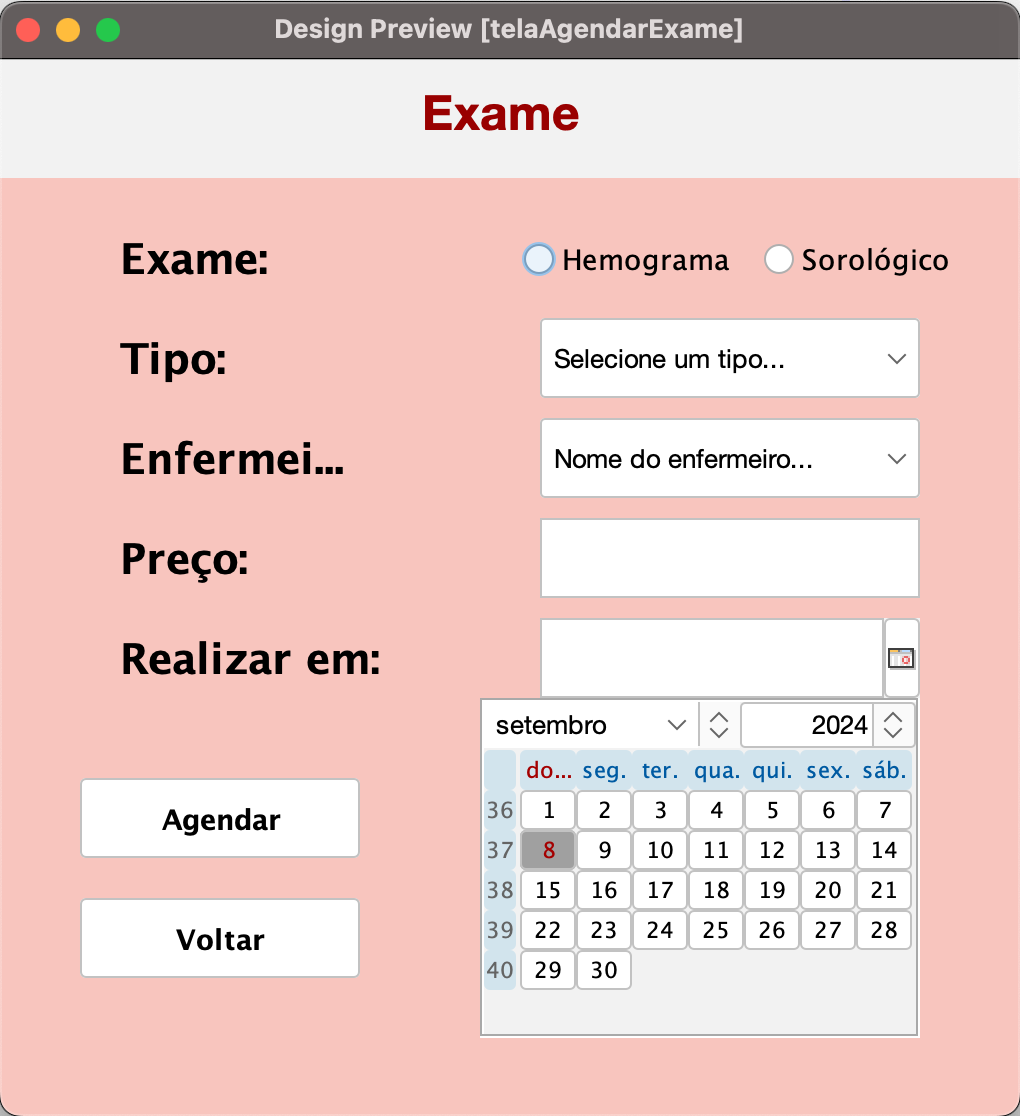
\includegraphics[width=6cm]{telaAgendarExame.png}
            \caption{Tela Agendar Exame}
        \end{figure}

        A tela Agendar Exame facilita o preenchimento dos dados necessários para o agendamento de exames, permitindo: definir o tipo, o exame específico, o enfermeiro responsável e a data de realização, e visualizar o preço.
        
        \begin{figure}[H]
            \centering
            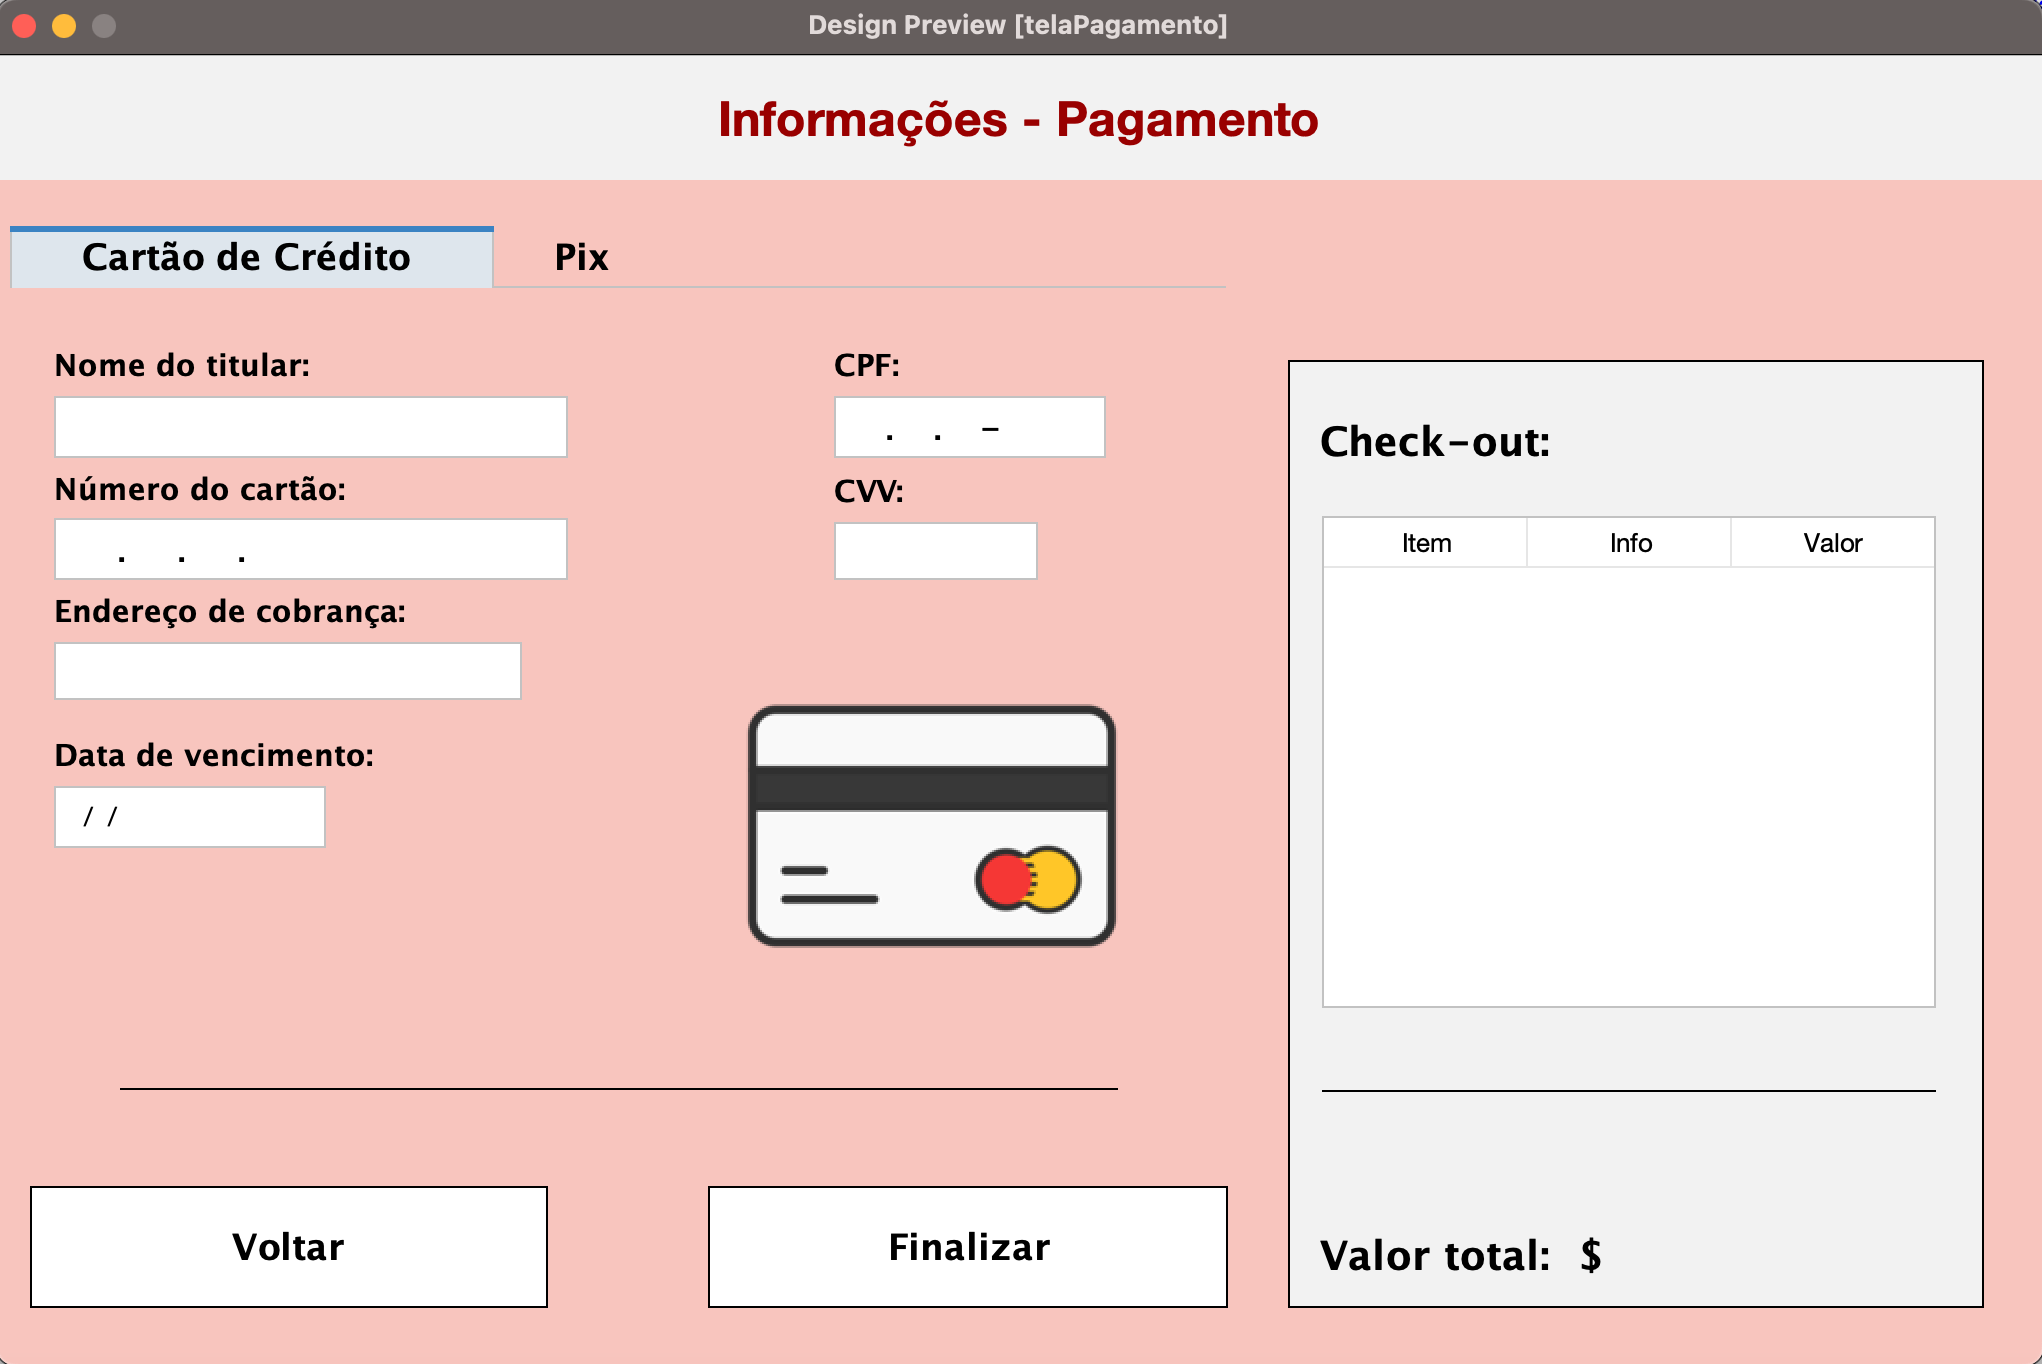
\includegraphics[width=8cm]{telaPagamento.png}
            \caption{Tela Pagamento}
            \label{Figure 14}
        \end{figure}

        A tela Pagamento encerra o fluxo de criação e organização dos agendamentos, disponibilizando campos para preencher dados da forma de pagamento escolhida, visualização do valor final, com ou sem desconto.
        
    \end{multicols}

\subsection{Parte Enfermeiro}

    \vspace{14mm}
    \begin{figure}[H]
        \centering
        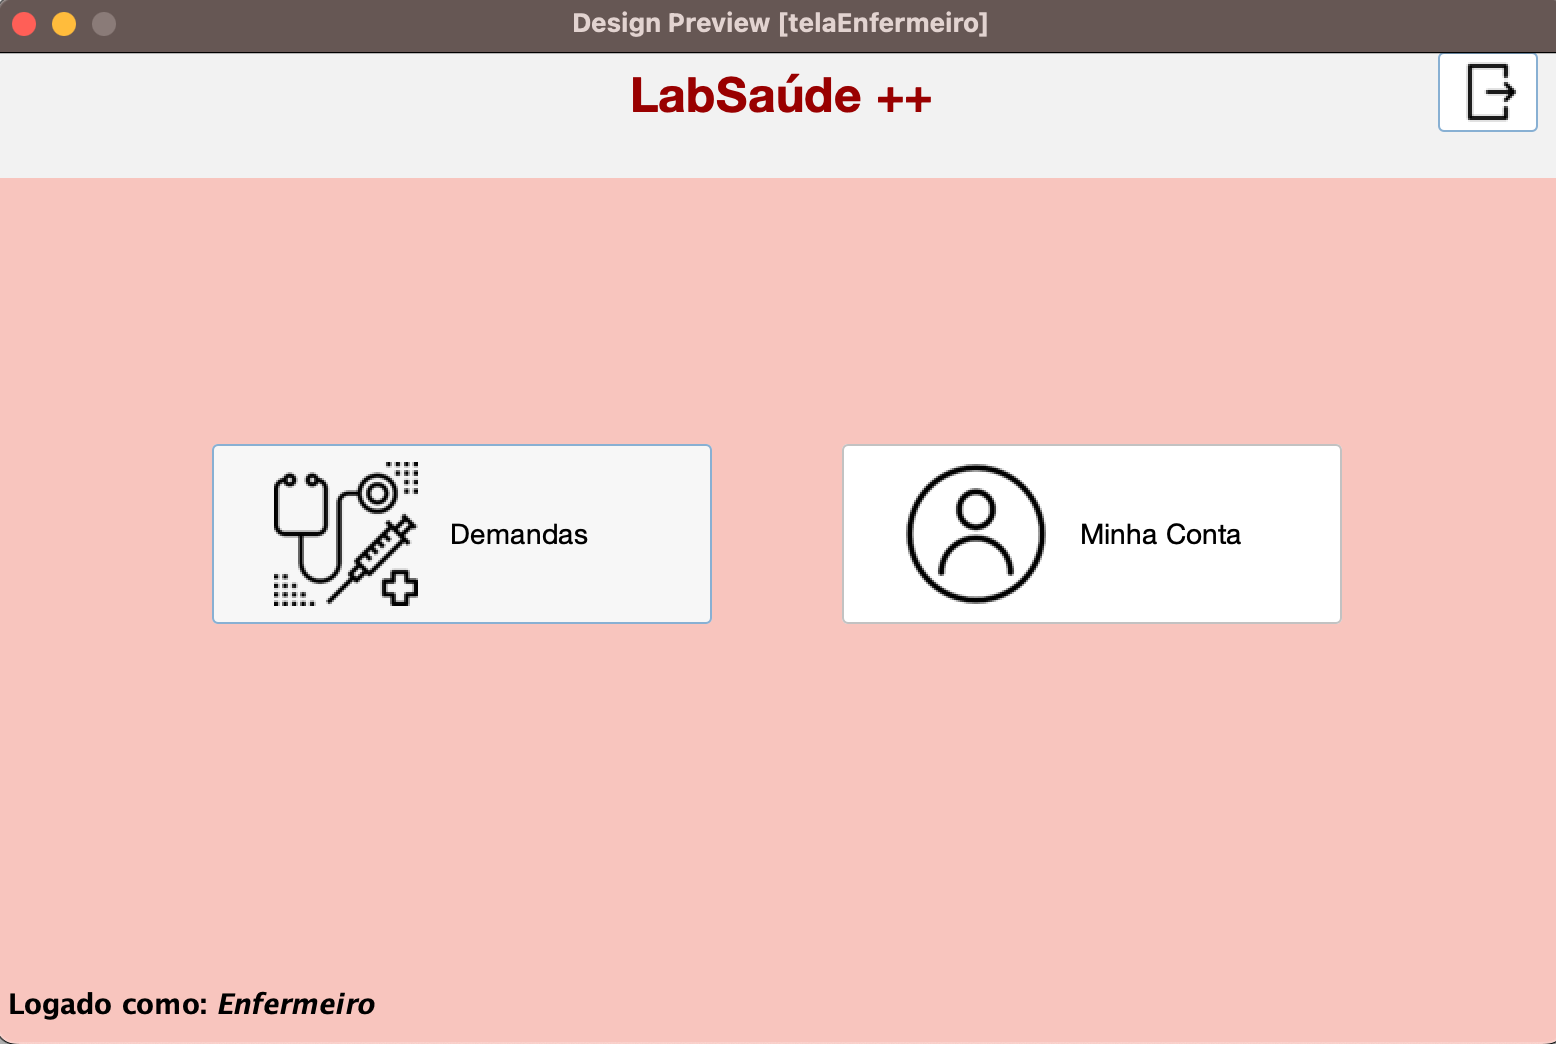
\includegraphics[width=10cm]{telaEnfermeiro.png}
        \caption{Tela Enfermeiro}
    \end{figure}
    
    Essa tela é responsável pela conexão das principais funções do usuário Enfermeiro, que são: visualizar as demandas e os resultados, realizar exames e aplicar vacinas, e alterar os dados da própria conta.
    
    \begin{multicols}{2}
        
        \begin{figure}[H]
            \centering
            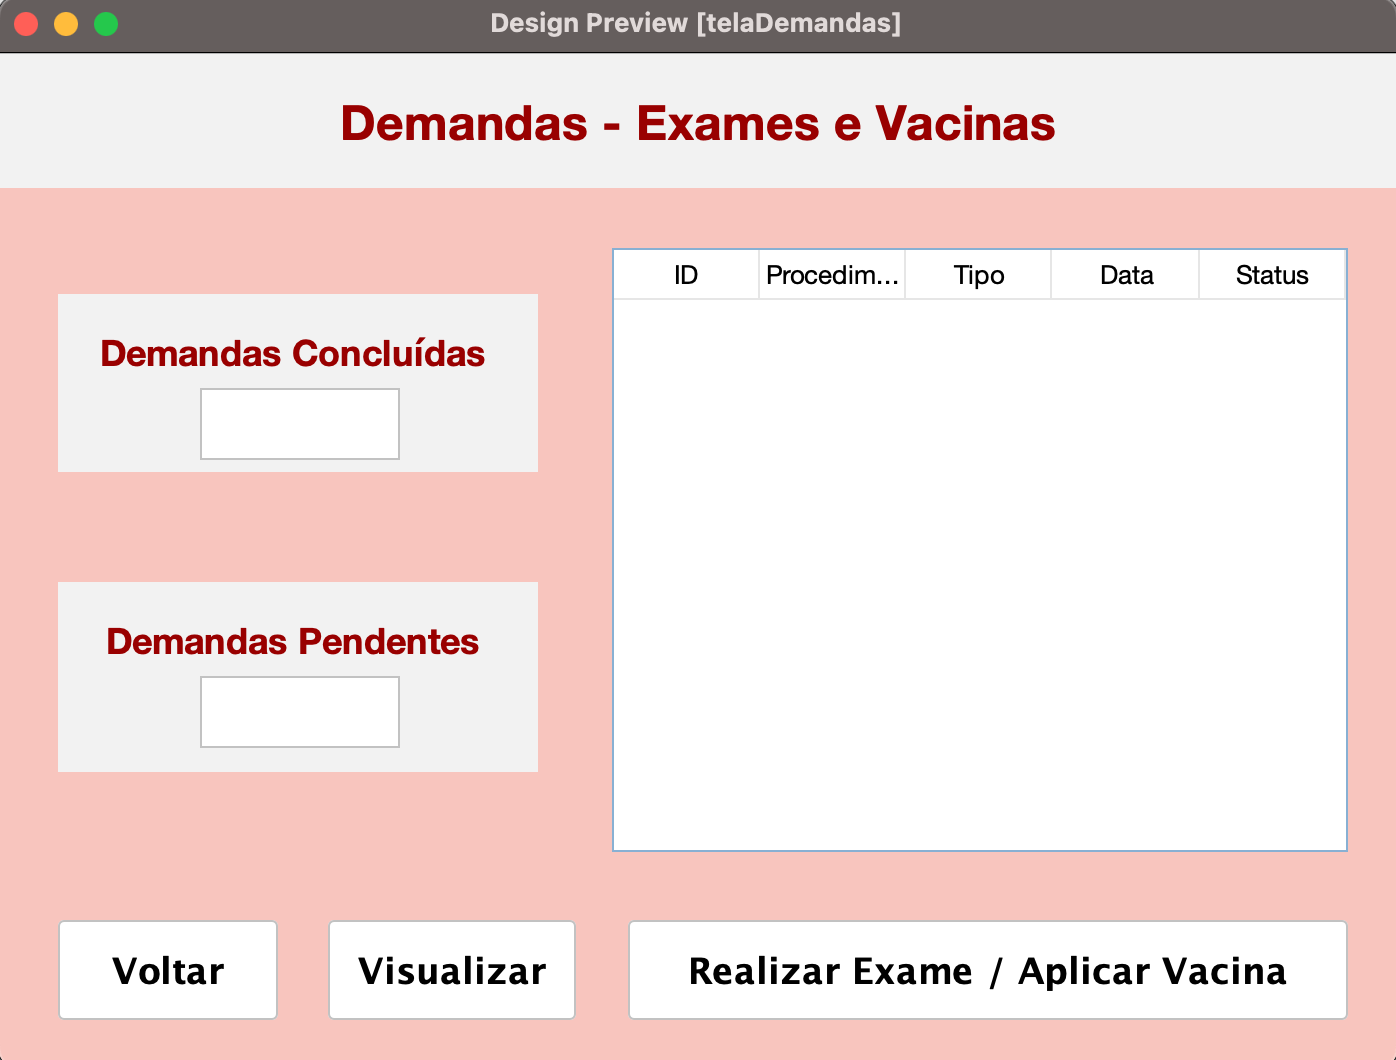
\includegraphics[width=8cm]{telaDemandas.png}
            \caption{Tela Demandas}
            \label{Figure 16}
        \end{figure}
        
        Essa tela uni os agendamentos cadastrados para o enfermeiro logado, permitindo que ele acesse suas demandas, concluídas ou pendentes. Além de, poder visualizar o resultado das demandas já finalizadas.
        
        \begin{figure}[H]
            \centering
            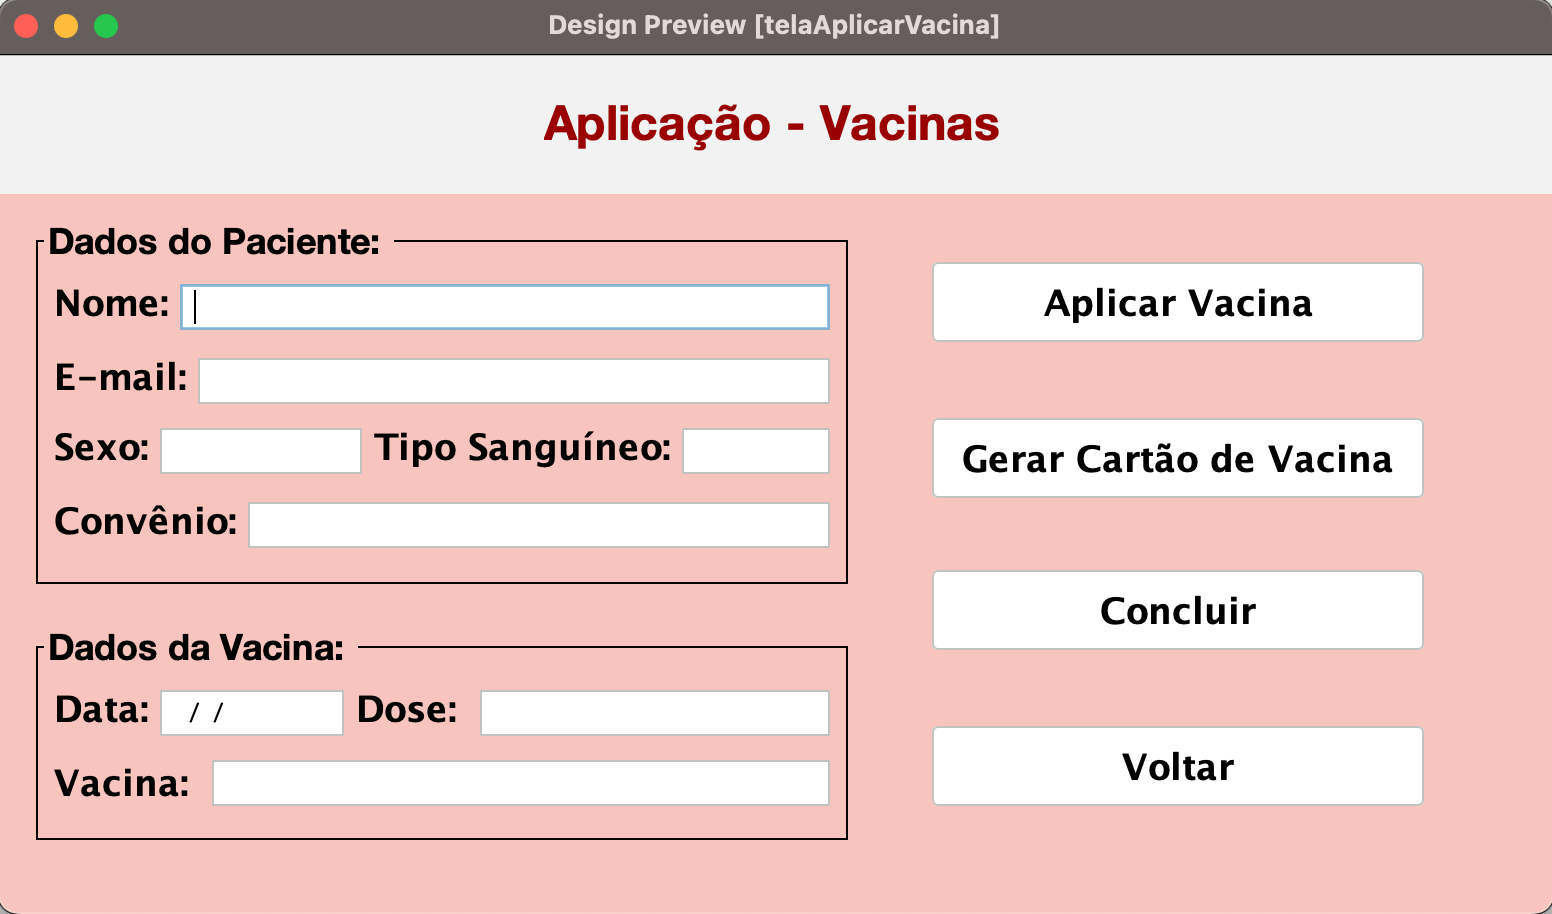
\includegraphics[width=8cm]{telaAplicarVacina.png}
            \caption{Tela Aplicação Vacina}
        \end{figure}

        A tela Aplicação Vacina possibilita ao enfermeiro: visualizar os dados relevantes do paciente e da vacina, aplicar a dose - fazendo uma dedução do estoque, gerar o Cartão de Vacina - comprovando a aplicação, e concluir a demanda atualizando a tela anterior - Tela Demandas (\ref{Figure 16}).
        
        \begin{figure}[H]
            \centering
            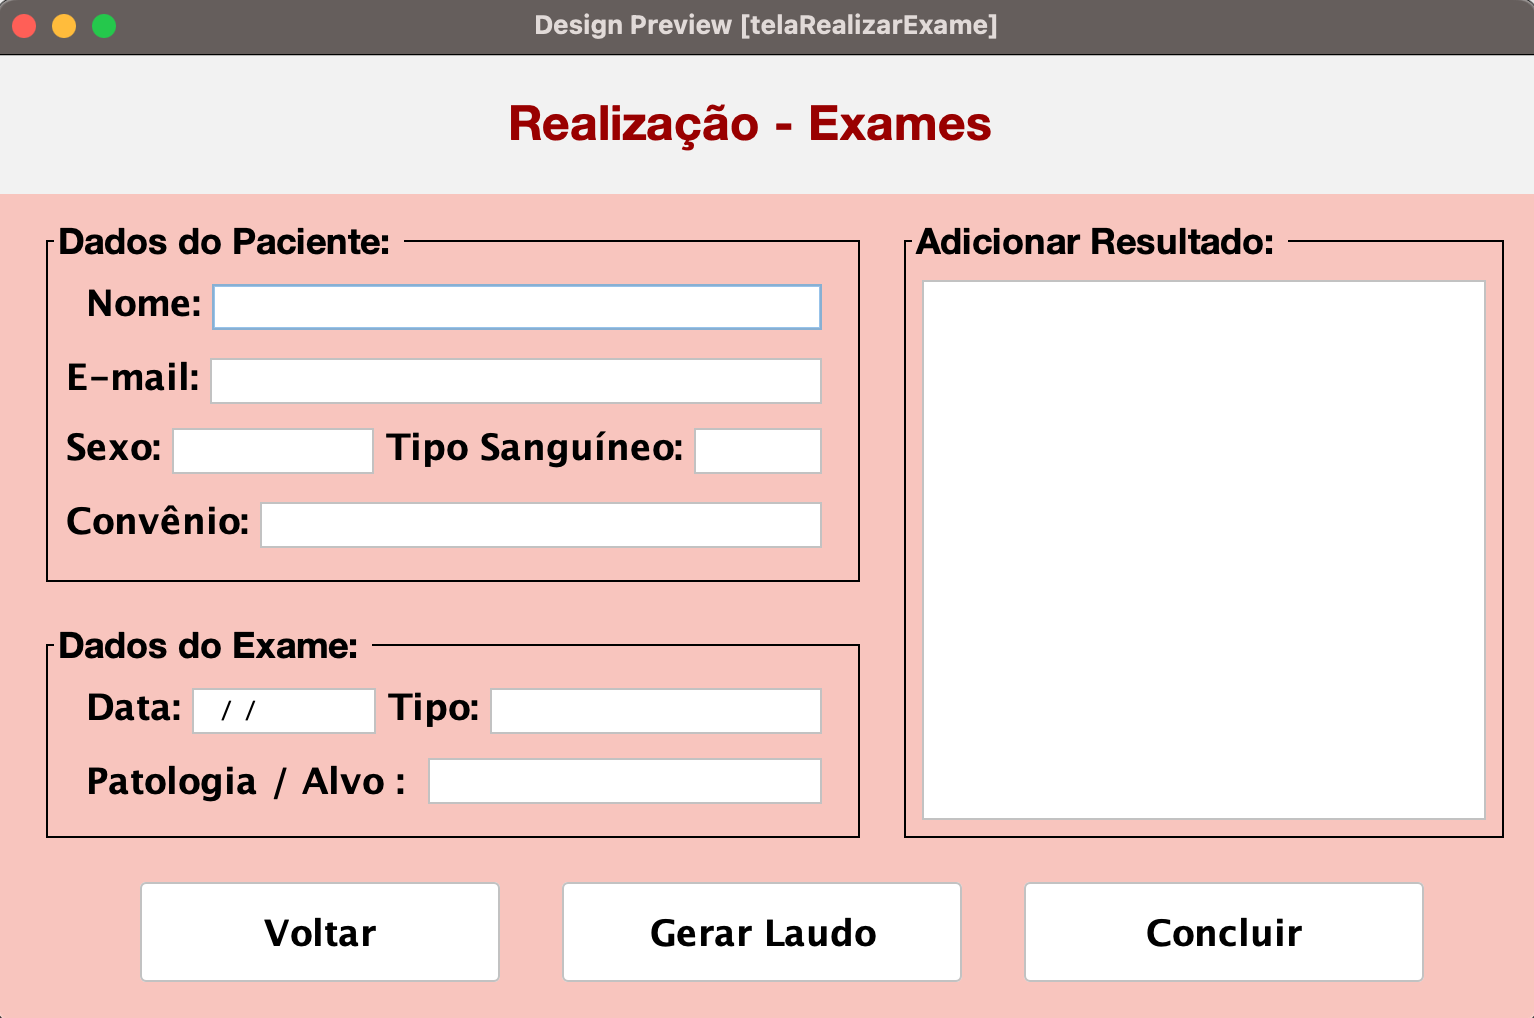
\includegraphics[width=8cm]{telaRealizarExame.png}
            \caption{Tela Realização Exame}
        \end{figure}

        A tela Realização Exame possibilita ao enfermeiro: visualizar os dados relevantes do paciente e do exame, adicionar um resultado, gerar um laudo, e concluir a demanda atualizando a tela anterior - Tela Demandas (\ref{Figure 16}).
        
        \begin{figure}[H]
            \centering
            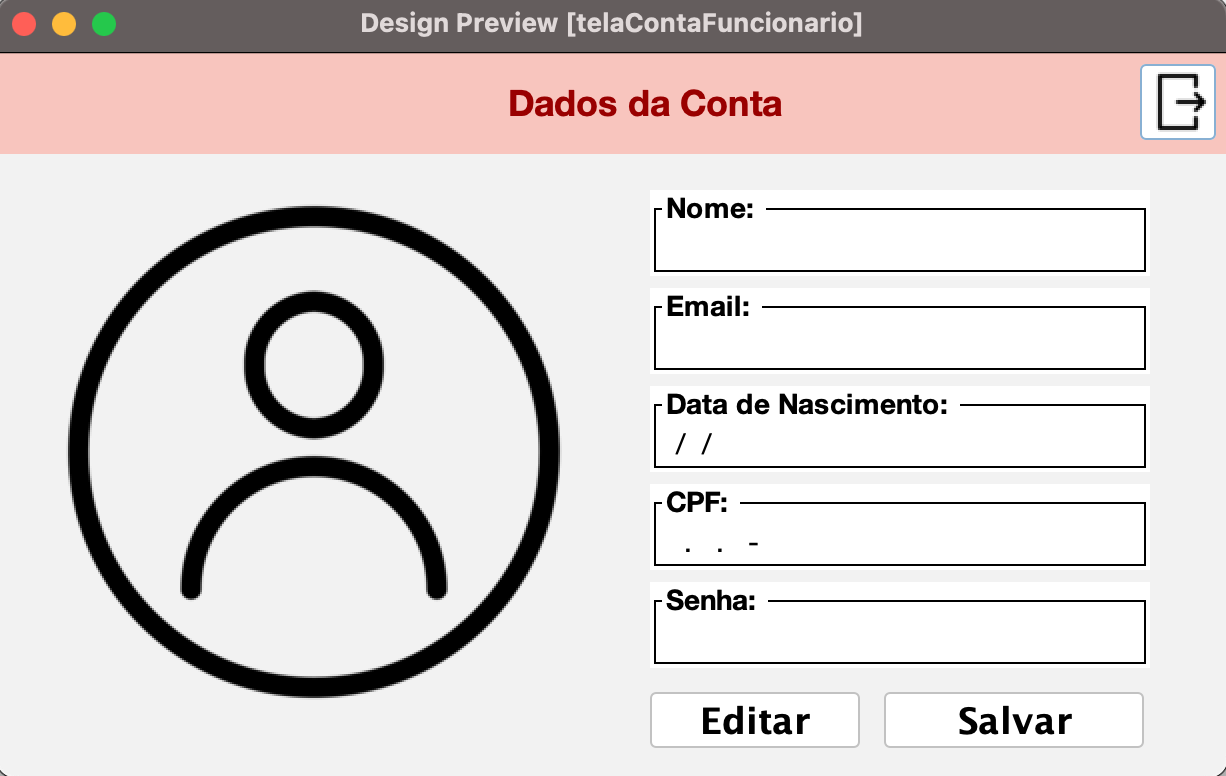
\includegraphics[width=8cm]{telaContaFuncionario.png}
            \caption{Tela Conta Funcionário}
            \label{Figure 19}
        \end{figure}

        A tela Conta Funcionário permite ao usuário logado visualizar seus dados básicos e alterá-los - salvando no banco de dados, a depender da necessidade.
        
    \end{multicols}

\section{Organização dos Exames e vacinas}
    \vspace{10mm}
    A seguir, apresentamos tabelas com os exames e vacinas oferecidos pela clínica.

    \subsection{Exames de Sangue}
        \begin{table}[H]
            \centering
            \caption{Exames de Sangue e suas respectivas informações e preços.}
            \label{tab:exames de sangue}
            \begin{tabular}{|c|c|c|}
            \hline
            Nome do Exame & Informações & Preços em reais \\
            \hline
            Hemograma & Contagem de leucócitos, hemácias e plaquetas & 75,00\\
            \hline
            Colesterol & Análise de VLDL, LDL e HDL & 60,00 \\
            \hline
            Glicemia & Análise do nível de glicose no sangue & 30,00 \\
            \hline              
            Ácido Úrico & Análise do nível de ácido úrico no sangue & 32,00 \\
            \hline
            Creatina & Análise do nível de creatinina no sangue & 45,00 \\
            \hline
            \end{tabular}
        \end{table}

        A Tabela \ref{tab:exames de sangue} apresenta uma lista de exames de sangue oferecidos pela clínica, detalhando informações específicas sobre cada exame e seus respectivos preços. Os exames incluem desde análises completas como o hemograma, até medições de colesterol, glicemia, ácido úrico e creatinina, permitindo diagnósticos e monitoramentos essenciais para a saúde do paciente.
    
    \subsection{Exames Sorológicos}

        \vspace{10mm}
        \begin{table}[H]
            \centering
            \caption{Exames sorológicos e seus respectivos preços.}
            \label{tab:exames sorológicos}
            \begin{tabular}{|c|c|c|}
            \hline
            Nome do Exame & Preços em reais \\
            \hline
            Dengue & 35,00\\
            \hline
            Zika Vírus & 30,00 \\
            \hline
            Covid-19 & 15,00 \\
            \hline
            Sífilis & 18,00 \\
            \hline
            Rubéola & 32,00 \\
            \hline
            Toxoplasmose & 25,00 \\
            \hline
            HIV & 20,00 \\
            \hline
            Hepatites A, B, C, D e E & 20,00 \\
            \hline
            \end{tabular}
        \end{table}

        A Tabela \ref{tab:exames sorológicos} apresenta os exames sorológicos disponíveis na clínica, juntamente com seus respectivos preços. Estes exames são importantes para a detecção de doenças como Dengue, Zika vírus, HIV, Hepatites e outras infecções, auxiliando no diagnóstico precoce e no tratamento adequado dos pacientes.

    \subsection{Vacinas}
        \begin{table}[H]
            \centering
            \caption{Vacinas e suas respectivas informações e preços.}
            \label{tab:vacinas}
            \begin{tabular}{|c|c|c|}
            \hline
            Nome da Vacina & Informações & Preços em reais \\
            \hline
            Tríplice Viral & Protege contra sarampo, caxumba e rubéola - 2 doses & 90,00\\
            \hline
            Hepatite B & Protege contra hepatite B - 3 doses & 84,00 \\
            \hline
            Dupla Adulto & Protege contra tétano e difteria - 1 dose a cada 10 anos & 135,00 \\
            \hline
            Febre Amarela & Protege contra febre-amarela - 1 dose & 112,00 \\
            \hline
            Meningocócica ACWY & Protege contra a meningite - 1 dose & 250,00 \\
            \hline
            HPV & Protege contra o câncer de colo de útero - 3 doses & 75,00 \\
            \hline
            \end{tabular}
        \end{table}

        A Tabela \ref{tab:vacinas} apresenta uma lista de vacinas oferecidas pela clínica, com detalhes sobre as doenças que elas previnem, o número de doses recomendadas e os preços. Entre as vacinas listadas estão a Tríplice Viral, Hepatite B, Dupla Adulto, e outras, cada uma com suas respectivas informações e custo.

        \vspace{20mm}

        \section{Referências}

            \bibliographystyle{sbc}
            \bibliography{relatorio}  
            Paul Deitel, Java Como Programar, 1993
            \\
            \href{https://www.youtube.com/playlist?list=PLHz_AreHm4dkI2ZdjTwZA4mPMxWTfNSpR}{Curso em vídeo - Gustavo Guanabara, Curso de Java para Iniciantes}
            \\
            Geek for Geeks, Introduction to Java Swing
            \\
             \href{https://jar-download.com/artifacts/com.itextpdf/itextpdf/5.5.9/source-code}{iTextPDF} - Biblioteca para manipulações de PDF, 5.5.9 
            \\
            \href{https://www.youtube.com/watch?v=4c3WYK5FpqI&t=463s&ab_channel=techfort}{tech fort, How to install add JDateChooser, JCalendar Date Picker in netbeans IDE Swing}
            \\
            \href{https://chatgpt.com/}{ChatGPT}
            \\

\end{document}